%% Generated by build.py from the Markdown files in Manuscript/draft/ -- do not edit by hand.
%% Springer Nature LaTeX template v3.1 (sn-jnl.cls), Vancouver numbered references, for BMC Psychiatry.
\documentclass[pdflatex,sn-vancouver-num]{sn-jnl}

\usepackage{graphicx}%
\usepackage{multirow}%
\usepackage{amsmath,amssymb,amsfonts}%
\usepackage{amsthm}%
\usepackage{mathrsfs}%
\usepackage[title]{appendix}%
\usepackage{xcolor}%
\usepackage{textcomp}%
\usepackage{manyfoot}%
\usepackage{booktabs}%
\usepackage{longtable,array,calc}% tables written by pandoc
\usepackage{url}%
\providecommand{\tightlist}{\setlength{\itemsep}{0pt}\setlength{\parskip}{0pt}}
\makeatletter\providecommand{\real}[1]{#1}\makeatother
\DeclareUnicodeCharacter{00A7}{\S{}}
\DeclareUnicodeCharacter{00B1}{\ensuremath{\pm}}
\DeclareUnicodeCharacter{00B2}{\textsuperscript{2}}
\DeclareUnicodeCharacter{00D7}{\ensuremath{\times}}
\DeclareUnicodeCharacter{00E4}{\"a}
\DeclareUnicodeCharacter{0394}{\ensuremath{\Delta}}
\DeclareUnicodeCharacter{03B2}{\ensuremath{\beta}}
\DeclareUnicodeCharacter{03B3}{\ensuremath{\gamma}}
\DeclareUnicodeCharacter{03B4}{\ensuremath{\delta}}
\DeclareUnicodeCharacter{03C1}{\ensuremath{\rho}}
\DeclareUnicodeCharacter{2013}{--}
\DeclareUnicodeCharacter{2014}{---}
\DeclareUnicodeCharacter{2019}{'}
\DeclareUnicodeCharacter{2026}{\ldots{}}
\DeclareUnicodeCharacter{2074}{\textsuperscript{4}}
\DeclareUnicodeCharacter{2075}{\textsuperscript{5}}
\DeclareUnicodeCharacter{207B}{\textsuperscript{--}}
\DeclareUnicodeCharacter{2212}{\ensuremath{-}}
\DeclareUnicodeCharacter{2264}{\ensuremath{\leq}}
\DeclareUnicodeCharacter{2265}{\ensuremath{\geq}}

\raggedbottom

\begin{document}
\title[Deep fusion vs mixed models for adolescent psychopathology]{Does deep cross-modal fusion improve prediction of late-adolescent psychopathology? A comparison with mixed-effects models in a Swedish twin cohort}

\author[1]{\fnm{Silpa Soni} \sur{Nallacheruvu}}\email{\textcolor{red}{[AUTHOR INPUT: email]}}
\author[1]{\fnm{Shuyang} \sur{Yao}}\email{shuyang.yao@ki.se}
\author[1]{\fnm{Sam} \sur{Andersson}}\email{sam.andersson@ki.se}
\author[1]{\fnm{Tong} \sur{Gong}}\email{tong.gong@ki.se}
\author[1]{\fnm{Lu} \sur{Yi}}\email{lu.yi@ki.se}
\affil[1]{\orgname{\textcolor{red}{[AUTHOR INPUT: affiliations and corresponding author]}}}

\abstract{% src: 04_results.md (prediction_metrics_summary.csv, paired_comparisons.csv, ML_comparators_tuning.csv). Word count without headings: 348 (2026-10-25). 

\textbf{Background:} Deep multimodal fusion networks can model interactions between psychiatric risk domains, but whether they predict better than well-specified regression models is rarely tested on identical data. We compared a deep cross-modal fusion network, which fuses adolescent substance use with each other risk domain, against regression and machine-learning models.

\textbf{Methods:} We analysed 4,033 twins (2,690 pairs) from the Child and Adolescent Twin Study in Sweden with complete data on 105 predictors in 11 groups, including substance use at age 15, neurodevelopmental traits, adverse experiences and 16 cell-type-specific polygenic scores. Outcomes were continuous scores of psychotic-like and hypomanic experiences and of depressive symptoms at age 18. Comparators were generalised linear and additive mixed models (GLMM, GAMM) with a twin-pair random intercept and 24 substance-use interactions mirroring the fusion design, and linear regression, an elastic net and gradient boosting tuned within the training data. All models were evaluated on the same five twin-pair-grouped splits, with corrected resampled t-tests. Secondary analyses covered calibration, sex, predictors measured by age 15, and the network's gate values.

\textbf{Results:} For psychotic-like and hypomanic experiences, mean test R² was 0.206 for the network, 0.228 for the GLMM and 0.227 for the GAMM; for depressive symptoms, it was 0.198, 0.202 and 0.200. No paired difference was statistically significant. An elastic net did best (0.260 and 0.237) and was ahead of the network on every split, but no difference survived correction. No interaction term survived correction. Without age-18 predictors, R² fell by 0.05--0.07 in every model. The network's gate values were nearly uniform and agreed poorly with SHAP values and permutation importance.

\textbf{Conclusions:} In this twin cohort, the fusion network did not predict better than mixed-effects models with matched inputs and interactions, even though part of its configuration was chosen using test data, and simpler models tuned on training data alone did better. The data gave little evidence of interactions between adolescent substance use and other risk domains, and the network's gates did not indicate predictor importance. Deep psychiatric prediction models should be benchmarked against well-specified regression models on identical splits before their complexity or attention-based explanations are relied on.}

\keywords{Psychotic-like experiences, Depressive symptoms, Adolescent substance use, Polygenic risk scores, Deep learning, Multimodal fusion, Mixed-effects models, Prediction model, Twin study}

\maketitle
%% ---------------- 02_background.md ----------------
% STATUS 2026-10-25: Background for BMC Psychiatry (replaces 02_introduction.md, written for AIIM). Gap statement rewritten with the L-02 studies (reference_registry.md §G).
% - BMC research articles open with "Background"; the template asks for no subheadings in this section.
% - Framing: neutral benchmark (DCMFNet vs matched mixed models) plus a check of attention-based explanations.
% The planted-interaction simulation, learning curves and stream ablation (E-16, E-14, E-06 ablation part) were
% not run and are not promised here.
% - Citations use pandoc keys [@R-...] from literature/reference_registry.md (and latex/references.bib).
% A key may support a claim only if its "Content access" covers it; otherwise [VERIFY: content].
% - Outcome labels are working labels pending M-01.

\section{Background}

Psychotic-like experiences, hypomanic symptoms and depressive symptoms are common in late adolescence. Most are transient, but they are not benign: in the cohort studied here, psychotic experiences in adolescence were associated with later substance use disorder and suicide attempts \citep{R-CEDERLOF}. Risk factors for these symptoms and for the psychotic disorders they may precede span several domains: substance use, particularly cannabis \citep{R-DIFORTI, R-HALL}; childhood adversity \citep{R-VARESE}; socioeconomic circumstances \citep{R-AGERBO}; and inherited liability captured by polygenic risk scores (PRS) \citep{R-PGC3}. % content checked 2026-10-26 (abstracts): R-DIFORTI and R-AGERBO concern psychotic disorder/schizophrenia, hence 'and for the psychotic disorders'; R-PGC3 is the SCZ GWAS underlying PRS 
Mapping psychiatric genetic signal onto specific brain cell types \citep{R-YAO2025} now allows cell-type-specific PRS, which may carry more targeted information than a genome-wide score.

A long-standing hypothesis holds that genetic and environmental risk factors act jointly rather than additively, although such interactions remain poorly understood \citep{R-ROBINSON}. Applied to the domains above, genetic liability or early adversity would change the effect of substance use. % R-ROBINSON abstract checked 2026-10-26: review of environmental risk factors (incl. cannabis, childhood adversity) and GxE for SCZ/BD 
If such interactions are strong, models that represent them should predict symptoms better than additive models. Deep multimodal fusion networks are one way to do this: they combine groups of inputs (``modalities'') through learned non-linear interactions, and they are increasingly applied to heterogeneous health data \citep{R-BORSOS}. A fusion architecture in which one exposure domain conditions the representation of every other domain, such as the iterative gated fusion of the Deep Cross-Modal Fusion Network (DCMFNet) \citep{R-DCMF}, matches the interaction hypothesis directly. Such networks also contain attention-like gates, which are often read as indicators of which inputs matter.

Matching the hypothesis does not guarantee better predictions. In clinical prediction, a systematic review found no performance benefit of machine learning over logistic regression in comparisons at low risk of bias, and calibration was rarely assessed \citep{R-CHRIST}. On medium-sized tabular data, tree ensembles usually outperform deep networks \citep{R-GRIN}. Studies of adolescent mental health point the same way:
- \textbf{In the cohort used here,} random forests, support vector machines, gradient boosting and a neural network predicted mental-health problems at age 15 no better than logistic regression \citep{R-TATE}.
- \textbf{In a US cohort,} gradient boosting improved the prediction of depressive symptoms over logistic regression only slightly, and polygenic scores added nothing to environmental predictors \citep{R-GEURGAS}.
- \textbf{For psychotic experiences in adolescents,} polygenic and polyenvironmental risk scores did not predict the outcome \citep{R-NAVARRO}.
- \textbf{In a large child cohort,} earlier symptoms were the strongest predictors of later mental-health problems, and neuroimaging added little \citep{R-HOU}.

Where multimodal prediction of psychosis has worked well, in patients at clinical high risk, separate clinical, polygenic and imaging models were combined step by step rather than fused within one network \citep{R-KOUTS}.

To our knowledge, no study has tested whether a deep fusion network built around substance-use interactions, using polygenic and environmental predictors in a population cohort, predicts better than regression models given the same inputs and interactions. % VERIFIED 2026-10-28 (L-02): PubMed search, title/abstract blocks for deep/fusion models (deep learning, neural network*, multimodal/multi-modal fusion, multimodal deep, cross-modal, attention mechanism*) × psychotic/hypomanic/depressive outcomes × PRS/substance use/cannabis × adolescent/youth/cohort/twin: 9 hits; adding a regression/mixed-model block gave 2 (both among the 9). Closest records read in full by the author (PMIDs 41399528, 36411277, 34899225): none tested this comparison. Non-systematic search. 
Such a test also has to avoid artefacts that favour the more flexible model:
- model selection on test data;
- feature screening outside the training data \citep{R-KAPOOR};
- related individuals on both sides of a split \citep{R-ROBERTS};
- unequal tuning effort;
- comparators that lack the interactions the flexible model is credited with.

Finally, attention weights are not necessarily faithful explanations of a model's predictions \citep{R-JAIN}. Gate values therefore need to be checked against attribution methods that measure what the model relies on.

We therefore compared DCMFNet, adapted so that substance use at age 15 is fused with each other risk domain, against two kinds of comparator:
- linear and generalised additive mixed models given the same predictors, a twin-pair random intercept and interaction terms that mirror the network's fusion design;
- three standard machine-learning models (linear regression, an elastic net and gradient boosting) tuned within the training data.

All models were evaluated on identical twin-pair-grouped splits in the Child and Adolescent Twin Study in Sweden \citep{R-CATSS}, with outcomes at age 18. We asked:
1. whether the fusion network predicted better than these comparators, including calibration, performance by sex and models restricted to predictors measured by age 15;
2. whether the mixed models showed evidence of the substance-use interactions that motivate the fusion design;
3. whether the network's attention gates agreed with SHAP values and permutation importance computed on the same models, and with exact SHAP values from the mixed models.

% Do NOT add: superiority claims; "interpretable" claims based on gate values (D-12); causal or "amplifier" language. 
%% ---------------- 03_methods.md ----------------
% STATUS 2026-10-23: Methods for BMC Psychiatry (replaces 03_materials_and_methods.md, written for AIIM).
% - Describes the analysis as it is now run: shared splits, updated GLMM/GAMM (E-01, E-02 completed 2026-10-23),
% prediction-level evaluation, age-15 sensitivity analysis and attribution analyses (scripts written 2026-10-23;
% outputs pending from the author's runs).
% - DCMFNet configuration selection is described as conducted, with the test-data involvement disclosed (D-04, D-09, D-21;
% E-03 not run). The ML benchmark is described as conducted.
% - BMC allows topical subheadings in Methods. Section numbers are not used (BMC style).
% - Outcome labels follow D-03 (descriptive names) pending author confirmation (M-01).

\section{Methods}

\subsection{Study population}

We used data from the Child and Adolescent Twin Study in Sweden (CATSS), an ongoing population-based cohort of all twins born in Sweden since July 1992, identified through the Swedish Twin Registry. Parents are interviewed by telephone about their children's health around the twins' 9th or 12th birthday, and twins and parents complete questionnaires at ages 15 and 18 \citep{R-CATSS}. % src: Thesis Report §3.1 p.7; Anckarsäter et al. 2011 abstract (PMID 22506305, read 2026-10-28): all twins born in Sweden since 1 July 1992; parental interviews at the 9th or 12th birthday since 2004; questionnaires to twins and parents at 15 and 18. Response rates not stated here (80% for the age-9/12 interviews up to 2010 only). 
We used the neurodevelopmental measures from the age-9 parent interview, self-reports at ages 15 and 18, and genotype data available for a subset of participants. % informant verified 2026-10-28 from Anckarsäter et al. 2011 (parental telephone interview at 9/12) 
The analysis data were prepared by the research team (files last updated in November 2023) and analysed on a secure server at Karolinska Institutet between November 2025 and October 2026. % author, 2026-10-28: original data files last modified 2023-11-23; access started by 2025-11-06 at the latest; access ends about 2026-10-28 
\textcolor{red}{{[}AUTHOR INPUT: years in which the age-15 and age-18 questionnaires used here were collected, and birth years covered (M-06); from the research team or CATSS documentation{]}}

Individuals were eligible if they had substance-use data at age 15 and outcome data at age 18. The analysis sample comprised all eligible individuals with complete data on every predictor and both outcomes: 4,033 individuals from 2,690 twin pairs. The sample size was set by the available data; no formal sample size calculation was made. % src: Models/DCMFNet/Results/Final Best Model/best_model_training.log:1-3 (shape (4033, 125); 2,017 + 673 = 2,690 cmpair IDs) 
Of the 13,146 CATSS twins in the study data, 9,261 had data on substance use at age 15 and on both outcomes at age 18 and were eligible. Participant flow is shown in Fig. 1. % src: thesis Figs 3.1 and 3.3 (13,146; 3,885 excluded for missing exposure or outcome), author confirmed 2026-10-28 (W-02); 9,261 = rows of catss_final_data.csv (analysis_sample_flow.csv). Thesis Fig. 3.1 reports 9,160 genotyped among the 13,146; 6,643 of the 9,261 eligible have PRS (analysis_sample_flow.csv), so about 2,500 genotyped twins lacked substance use at 15 or an outcome. The two numbers have different denominators and do not conflict. 
We compared the analysis sample with excluded eligible participants on sex, outcomes, substance use at age 15 and summary scores of each predictor group, using standardised mean differences (Table 1). Counts below five are not reported. % src: Data Preprocessing/Data Visualisation/analysis_sample_descriptives.R 

\subsection{Outcomes}

Two continuous outcomes were derived from self-report items at age 18. % src: Data Preprocessing/Data Analysis/catss_analysis_final.html, CATSS18 section (ple_var_list18, mdq_cmrs_list18, cesd_var_list18 and their response labels), read 2026-10-28; outcome item lists in rename_catss_with_mapping.py:73-81 

\begin{itemize}
\tightlist
\item
  \textbf{Psychotic-like and hypomanic experiences (PLE-HM):} sum of 24 items, divided by 46: 7 items on psychotic-like experiences (for example feeling spied upon or seeing things that others cannot) from the Adolescent Psychotic-Like Symptom Screener \citep{R-LAURENS, R-APSS}, the 13 symptom items of the Mood Disorder Questionnaire \citep{R-MDQ} and 4 items from the Child Mania Rating Scale \citep{R-CMRS} (unrealistic abilities, talking fast, sexually inappropriate behaviour and hearing voices). % src: catss_analysis_final.html (ple_var_list18: spied, read_thoughts, Special_messages, special_powers, under_control_special, read_others_mind, seen_hallucinations; mdq_cmrs_list18: 13 MDQ items + unrealistic_abilities, talk_fast, sexual_inappropriate, hear_voices) 
  Psychotic-like and Child Mania Rating Scale items were scored from 0 to 3 and Mood Disorder Questionnaire items as no (0) or yes (1), so 46 is the maximum score. % author confirmed 2026-10-28: 7×3 + 13×1 + 4×3 = 46; instruments confirmed (M-01) 
\item
  \textbf{Depressive symptoms (DEP):} sum of the 11 items of the short form of the Center for Epidemiologic Studies Depression Scale (CES-D) \citep{R-CESD, R-CESD11}, each scored from 0 (``not at all or almost not at all'') to 3 (``all the time or almost all the time''), divided by 33, the maximum score. % src: catss_analysis_final.html (cesd_var_list18, cesd_labels_list18 0–3); the 11 items match the Iowa short form (Kohout 1993) item for item 
  The two positively worded items (being happy and enjoying life) were reverse-coded. % author confirmed 2026-10-28 
\end{itemize}

Both scores lie between 0 and 1 and were analysed as continuous outcomes without clinical thresholds.

\subsection{Predictors}

The 105 predictors were organised into 11 groups defined before analysis (number of variables in parentheses; full list in Additional file 1: Table S4): % src: best_model_training.log:2 ; Models/DCMFNet/Method/legacy/train.py:74-87 

\begin{enumerate}
\def\labelenumi{\arabic{enumi}.}
\tightlist
\item
  Substance use at age 15 (SUD15; 6): frequency of cigarette, snus, alcohol, cannabis and non-medical painkiller use, and the maximum across other drug items. % src: Data Preprocessing/Feature Selection/feature_selection.py:76-97 
\item
  Polygenic risk scores (PRS; 16): a genome-wide schizophrenia PRS and cell-type-specific PRS restricted to genes specifically expressed in brain cell types of a human brain cell atlas \citep{R-SILETTI, R-YAO2025}, computed with PRS-CS \citep{R-PRSCS}. \textcolor{red}{{[}AUTHOR INPUT: GWAS summary statistics, LD reference, PRS-CS settings, genotyping platforms, imputation and QC --- TODO W-03{]}}
\item
  Psychotic-like, hypomanic and emotional symptoms at age 15 (SCZ15; 23).
\item
  ADHD symptoms at age 9 (ADHD9; 19).
\item
  Autism-related traits at age 9 (ASD9; 17). Groups 4 and 5 are the ADHD and autism-spectrum modules of the Autism--Tics, ADHD and other Comorbidities inventory (A-TAC), a parent telephone interview \citep{R-ATAC}. % author confirmed 2026-10-28 that the ADHD9 and ASD9 items are the A-TAC ADHD and autism modules; Larson et al. 2010 verified via Crossref/Europe PMC (PMC2823676) 
\item
  Adverse experiences at age 15 (ACE15; 7), mainly bullying victimisation.
\item
  Adverse experiences at age 18 (ACE18; 4): emotional abuse, hate crime, witnessing crime and other abuse or violence. % src: feature_selection.py:111-130 
\item
  Substance use at age 18 (SUD18; 4).
\item
  Parental socioeconomic indicators (SES; 4): parental education and country of birth.
\item
  Sex (1), as reported by parents in the opening questions of the age-9/12 interview. % author, 2026-10-28 (M-06) 
\item
  Genotyping batch × genetic principal component terms (4): products of batch indicators and the first two principal components, to adjust for population structure and batch effects. % src: rename_catss_with_mapping.py (add_batch_pc_interactions, pc_cols=['PC1','PC2']) 
\end{enumerate}

ACE18 and SUD18 were measured at the same assessment as the outcomes, so models that include them combine prospective and concurrent information. We therefore repeated all analyses without these groups (see \emph{Sensitivity analyses}).

\textbf{Variable screening.} The 236 candidate variables were reduced in four steps, guided by pairwise Pearson correlations and by SHAP values from LightGBM models fitted to each outcome \citep{R-LGBM, R-SHAP}. % src: Thesis §3.4 p.10-11 and Fig. 3.3; Data Preprocessing/Feature Selection/feature_selection.py; Data Analysis/Feature Importance/feature_importance.py 
1. Variables with more than 90\% missing values were removed. % src: feature_selection.py get_high_missingness_columns 
2. Groups of highly correlated items were combined into one variable by taking the highest response: 11 illicit-drug items into ``other drugs'' and beer into alcohol at age 15; six types of bullying at age 15; and five types of abuse or violence at age 18. % src: feature_selection.py group_columns (Drugs15, ACE15, ACE18) 
3. Parent-reported symptom items at age 18 were removed. They were highly correlated with the self-reports and had more missing values, so the outcomes are based on self-reports. % src: feature_selection.py group_columns (Symptoms18) 
4. A further 41 variables with 50--90\% missing values that could not be combined with correlated items were removed. Most were parent-reported items at age 15 or adverse experiences at age 9. % src: feature_selection.py drop_mid_missing_cols (41 variables: 30 parent-reported at 15, 8 at age 9, 3 at age 18) 

The LightGBM models used the outcomes and were fitted on random splits of the full sample (seeds 41--45) that do not correspond to the evaluation splits. % src: feature_importance.py:31-45, 104-112; D-09, E-04 
Although the reasons recorded in the code for each removal or grouping are missingness or correlation, the SHAP values informed these decisions, so we treat the screening as outcome-informed. Because all models received the same 105 predictors, this step could raise the performance of all models but does not favour any one of them. % E-04 resolved 2026-10-26: author confirmed screening was inferred from Pearson correlations and LightGBM SHAP values (thesis §3.4) 
Responses of ``don't know'' or ``don't want to answer'' were set to missing. % src: feature_selection.py:136-143 
No questionnaire item in the final data contained −1 or other negative codes. % src: missing_code_check.csv (no rows); A-03 resolved 2026-10-24 

\subsection{Data partitioning}

The data were split at the twin-pair level, so that co-twins were always in the same partition, into 75\% training and 25\% test sets. This was repeated with five random seeds (42--46). The same five splits were used for every model: the split identifiers were exported once and read by the R scripts. % src: Data Preprocessing/split_data.py; Models/GLMM/Method/GLMM_updated_split.R (read_split); legacy/train.py:61-68 
% checked 2026-10-25: Data Preprocessing/Data Analysis/split_summary.csv, matches_dcmfnet_log = True for seeds 42–46 
Each test set contained 998--1,028 individuals. % src: best_model_training.log:3, 361, 685, 1063, 1414 
For DCMFNet, a further pair-level 80/20 split of each training set formed a validation set for early stopping and learning-rate scheduling. % src: legacy/train.py:145-152 

\subsection{Deep cross-modal fusion network}

We adapted DCMFNet \citep{R-DCMF}, originally proposed for fusing image and text representations through iterative gated fusion (IGF), to grouped tabular predictors (Fig. 2). Substance use at age 15 is the anchor group. Each of groups 2--10 is fused with the anchor in its own IGF block, and a parallel independent stream receives all raw inputs, including the batch × PC terms. % src: Models/DCMFNet/Method/dcmfnet/model.py:115-205; legacy/train.py:49, 74-87 

\textbf{Fusion block.} Let \(\mathbf{x}_a\) be the anchor features (\(d_a = 6\)) and \(\mathbf{x}_m\) the \(d_m\) features of group \(m\). Block \(m\) has depth \(L_m\) and starts from \(\mathbf{g}_m^{(0)} = \mathbf{x}_m\). For \(l = 1,\dots,L_m\):

\[\mathbf{f}_m^{(l)} = \tanh\big(\tanh(\mathbf{W}_1^{(l)}\mathbf{x}_a + \mathbf{b}_1^{(l)}) \odot \tanh(\mathbf{W}_2^{(l)}\mathbf{g}_m^{(l-1)} + \mathbf{b}_2^{(l)})\big), \tag{1}\]

\[\mathbf{z}_m^{(l)} = \sigma\big(\mathbf{W}_z^{(l)}(\mathbf{f}_m^{(l)} + \mathbf{g}_m^{(l-1)}) + \mathbf{b}_z^{(l)}\big), \tag{2}\]

\[\mathbf{g}_m^{(l)} = \tanh\big(\mathbf{W}_g^{(l)}[\mathbf{f}_m^{(l)};\, \mathbf{f}_m^{(l)} \odot \mathbf{z}_m^{(l)}] + \mathbf{b}_g^{(l)}\big), \tag{3}\]

where \(\sigma\) is the logistic function, \(\odot\) element-wise multiplication and \([\cdot;\cdot]\) concatenation. Equation 1 is a multiplicative interaction between the anchor and the current representation of group \(m\); Equations 2--3 form the gate of the original architecture. The block output concatenates the fused representations from all layers, \(\mathbf{u}_m = [\mathbf{f}_m^{(1)};\dots;\mathbf{f}_m^{(L_m)}]\). % src: dcmfnet/model.py:11-47, 106-112; thesis-era commit 6173d10 DCMFNet/model.py:38-101 

\textbf{Feature gating.} Each block output, the concatenated fused stream, the independent stream and the final representation pass through a feature gate

\[\phi(\mathbf{u}) = \mathbf{u} \odot \sigma\big(\mathbf{V}_2\, \mathrm{Dropout}(\mathrm{ReLU}(\mathbf{V}_1\mathbf{u} + \mathbf{c}_1)) + \mathbf{c}_2\big), \tag{4}\]

with hidden width \(\max(\lfloor D/r \rfloor, h_{\min})\) for input dimension \(D\). This gate was motivated by squeeze-and-excitation attention \citep{R-SE}, but it is computed for each individual from that individual's own features, without pooling. It is therefore an input-dependent weighting, not a population-level importance measure. % src: dcmfnet/model.py:50-77 — D-06 

\textbf{Streams and output.} The fused stream is \(\mathbf{h}_F = \phi_F([\phi_1(\mathbf{u}_1);\dots;\phi_9(\mathbf{u}_9)])\) and the independent stream is \(\mathbf{h}_I = \phi_I(\mathbf{x})\), where \(\mathbf{x}\) contains all 105 inputs. The prediction is \(\hat{y} = \mathbf{w}^\top \phi_{\mathrm{out}}([\mathbf{h}_F;\mathbf{h}_I]) + b\), with a linear output. % src: dcmfnet/model.py:168-205 
Because the independent stream feeds gated raw inputs to a linear output layer, the network contains an approximately additive pathway alongside the interaction pathway. Inputs were not standardised. % src: legacy/train.py:74-94 — D-13, E-07 

\textbf{Loss.} To give more weight to the sparse upper tail of the outcomes, we used a weighted Huber loss. Training outcomes were assigned to \(K\) equal-width bins on {[}0, 1{]}; each bin received a weight proportional to \(1/(n_k + 1)\), normalised to mean 1 and truncated at 20. Within each mini-batch, the weights were multiplied by a focal factor \((|y_i - \hat{y}_i| + 10^{-6})^{\gamma}\), computed without gradient, and renormalised to mean 1. % src: dcmfnet/losses.py:15-76; thesis-era 6173d10:DCMFNet/loss.py:60-73 — D-07 

\textbf{Training and configuration selection.} Networks were trained with the Adam optimiser \citep{R-ADAM}, weight decay, learning-rate reduction on plateau of the validation RMSE and early stopping with restoration of the best weights. % src: legacy/train.py:371-476 
Hyperparameters were selected with Optuna \citep{R-OPTUNA} (50 trials per outcome), minimising validation RMSE within the seed-42 training set (Additional file 1: Table S1, which also describes the tuning history). % src: git c49eec1:DCMFNet/tuning.py:49-71, 204-229 — D-21 
The search tuned one depth for all fusion blocks (best: 3 for PLE-HM, 2 for DEP). A subsequent sweep varied the depth of each block. For PLE-HM, the per-block depths from this sweep were adopted after per-block and uniform configurations had been compared on the test sets; for DEP, uniform depth 2 was kept (Additional file 1: Table S5). % src: Models/DCMFNet/Analysis/complexity_analysis.py:130-250; Results/Complexity Analysis/Pos_complexity_comparison.csv; git 5c35f0e, 6173d10 — D-04, D-05 
Several tuning runs were carried out, and the final choice among them was also informed by test-set results. % src: discrepancies.md D-21 (git history c49eec1 … 29 Apr) 
In addition, the seed-42 training data used for tuning overlap the test sets of seeds 43--46. % src: legacy/tuning.py:86-92, 216-217 — D-09 
All of these steps can only make DCMFNet's test performance optimistic relative to the comparators, which were not tuned. The selected hyperparameters are given in Table 2. % M-02 resolved 2026-10-26: author confirmed Table 2 matches hyperparameters.json (per-block PLE-HM configuration is the primary one) 

\begin{longtable}[]{@{}
  >{\raggedright\arraybackslash}p{(\linewidth - 4\tabcolsep) * \real{0.3333}}
  >{\raggedright\arraybackslash}p{(\linewidth - 4\tabcolsep) * \real{0.3333}}
  >{\raggedright\arraybackslash}p{(\linewidth - 4\tabcolsep) * \real{0.3333}}@{}}
\caption{Selected DCMFNet hyperparameters. % src: Models/DCMFNet/hyperparameters.json 
}\tabularnewline
\toprule\noalign{}
\begin{minipage}[b]{\linewidth}\raggedright
Hyperparameter
\end{minipage} & \begin{minipage}[b]{\linewidth}\raggedright
PLE-HM model
\end{minipage} & \begin{minipage}[b]{\linewidth}\raggedright
DEP model
\end{minipage} \\
\midrule\noalign{}
\endfirsthead
\toprule\noalign{}
\begin{minipage}[b]{\linewidth}\raggedright
Hyperparameter
\end{minipage} & \begin{minipage}[b]{\linewidth}\raggedright
PLE-HM model
\end{minipage} & \begin{minipage}[b]{\linewidth}\raggedright
DEP model
\end{minipage} \\
\midrule\noalign{}
\endhead
\bottomrule\noalign{}
\endlastfoot
Learning rate & 1.00 × 10⁻⁴ & 3.22 × 10⁻⁴ \\
Batch size & 4 & 6 \\
Maximum epochs & 23 & 20 \\
Weight decay & 2.95 × 10⁻⁵ & 1.79 × 10⁻⁴ \\
Fusion depth \(L_m\) (PRS, SCZ15, ADHD9, ASD9, ACE15, ACE18, SUD18, SES, Sex) & 5, 2, 1, 5, 4, 1, 1, 1, 5 & 2 (all blocks) \\
Dropout & 0.234 & 0.326 \\
Gate reduction ratio \(r\) / minimum width \(h_{\min}\) & 6 / 13 & 5 / 5 \\
Huber δ / focal γ / bins \(K\) & 0.086 / 1.32 / 13 & 0.116 / 2.62 / 10 \\
Scheduler patience / factor & 4 / 0.432 & 2 / 0.549 \\
Early-stopping patience & 5 & 7 \\
Trainable parameters & 105,501 & 71,623 \\
\end{longtable}

% src (parameter counts): recomputed 2026-10-26 by instantiating dcmfnet.model.DCMFNet with the hyperparameters.json values and sizes [6,16,23,19,17,7,4,4,4,1,4] (independent stream = all 105 inputs); 105,501 and 71,623, unchanged; no data used 

\subsection{Mixed-effects comparators}

\textbf{Generalised linear mixed model (GLMM).} The GLMM included all 105 predictors as linear main effects, a random intercept for twin pair and 24 interaction terms that mirror the network's fusion blocks: the SUD15 score multiplied by the score of each fused questionnaire group (SCZ15, ADHD9, ASD9, ACE15, ACE18, SUD18 and SES; 7 terms), by sex (1 term) and by each standardised PRS (16 terms). Group scores were the mean of the standardised items, standardised again; means and standard deviations were estimated in the training set and applied to the test set. % src: Models/GLMM/Method/GLMM_updated_split.R build_model_spec(), add_interaction_scores():96-111 
The model was fitted with \textcolor{red}{lme4::lmer} (Gaussian, identity link). % src: GLMM_updated_split.R:291-313 
With a Gaussian outcome and identity link, this GLMM is a linear mixed model. % Q-01 decided 2026-10-27: the author uses "GLMM" throughout 

\textbf{Generalised additive mixed model (GAMM).} The GAMM had the same specification, except that each PRS entered as a penalised smooth term and the twin-pair intercept as a random-effect smooth. It was fitted with \textcolor{red}{mgcv::gam} (Gaussian family, restricted maximum likelihood). Each smooth used mgcv's default thin-plate regression spline basis with dimension 10. % src: Models/GAMM/Method/GAMM_updated_split.R:25-29, 336, 356 (s(PRS) with no bs or k argument, so mgcv defaults: bs = 'tp', k = 10 for one covariate); mgcv 1.9-4 from versions_R.txt (V-04, 2026-10-28) 

For both models, test-set predictions were made at the population level, without the twin-pair random effect, because test pairs were not part of the training data. % src: GLMM_updated_split.R (predict re.form = NA); GAMM_updated_split.R (exclude = "s(cmpair)") 

\textbf{Machine-learning screening.} Forty regression algorithms from the LazyPredict list \citep{R-LAZY} were first fitted with scikit-learn default settings on the same splits and inputs (Additional file 1: Table S2). The estimators were called directly, without LazyPredict's own preprocessing, so inputs were not scaled. % src: Models/ML/Method/lazy_predict.py:82-111 (model_class() fitted on raw X; LazyRegressor not used); Models/ML/Results/{Pos,Neg}_benchmark_summary.csv 
Defaults suit some algorithms poorly. For example, the lasso with its default penalty predicted a constant. Ranking the screened models by test performance would also select on test data. The screening was therefore used only to describe how default-setting models perform.

\textbf{Tuned machine-learning comparators.} After the screening, we chose three comparators by model class, not by their rank in the screening:
- \textbf{linear regression} without penalty, which has nothing to tune;
- \textbf{an elastic net}, a penalised linear model that includes the lasso and ridge regression as special cases \citep{R-ZOU};
- \textbf{gradient-boosted trees}, which learn non-linear effects and interactions without a prespecified structure and are a strong benchmark for tabular data \citep{R-GRIN}.

For the elastic net, inputs were standardised, and the penalty strength (100 values) and L1 ratio (0.05--1) were chosen by cross-validation. For gradient boosting (scikit-learn \textcolor{red}{HistGradientBoostingRegressor}), 40 configurations were drawn at random over learning rate, number of trees, maximum depth, number of leaves, minimum leaf size and L2 penalty. Early stopping was not used, because its internal validation split is not grouped by twin pair. All tuning used the training split only, with five inner folds grouped by twin pair and mean squared error as the criterion. Each model was then refitted on the whole training split and evaluated once on the test split. The comparators used the same 105 inputs; in the age-15 analysis, ACE18 and SUD18 were removed. Like the network, they did not model twin dependence. % src: Models/ML/Method/ml_comparators_test_predictions.py (ELASTIC_NET_L1_RATIOS, BOOSTING_SPACE, N_BOOSTING_CONFIGS = 40, GroupKFold n_splits = 5); scikit-learn 1.8.0 from versions_python.txt 

\subsection{Evaluation and statistical comparison}

All models were evaluated on the same five test sets with the same metric code: the coefficient of determination, \(R^2 = 1 - \sum(y_i-\hat{y}_i)^2 / \sum(y_i-\bar{y})^2\), root-mean-squared error (RMSE), mean absolute error (MAE) and Spearman's rank correlation. Results are given as mean and standard deviation over the five splits. % src: Models/Model Comparison/prediction_evaluation.py core_metrics(), summarise() (ddof = 0); GLMM_updated_split.R header items 4–5 

Models were compared split by split with the corrected resampled t-test, which accounts for the overlap between training sets across splits \citep{R-NADEAU} (test-to-training ratio 1/3, 4 degrees of freedom), and 95\% confidence intervals for the mean differences were derived from the same corrected variance. P-values were adjusted with the Holm method within each metric, across all 18 comparisons among the network and the mixed models (three model pairs with each of two predictor sets, and full versus age-15-only predictors for each model, for both outcomes). Comparisons of the network with the three machine-learning comparators, and of each comparator's full and age-15-only predictor sets, formed a second family of 18 comparisons with its own Holm correction. % src: prediction_evaluation.py corrected_t_test(), holm() 
With five splits these tests have low power, so a non-significant difference is not evidence of equivalence.

For the mixed models, interaction terms were assessed with their Wald p-values, Holm-adjusted across the 24 terms, and PRS smooth terms by their effective degrees of freedom. % src: Models/GLMM/Results/{Pos,Neg}_GLMM_updated_all_coefs.csv; Models/GAMM/Results/GAMM_updated_{Pos,Neg}_smooth_terms.csv 

\subsection{Calibration, subgroup and sensitivity analyses}

The comparison was repeated with participant-level test predictions from DCMFNet retrained with the same seeds, splits and hyperparameters, so that all models were scored with identical code. % src: Models/DCMFNet/Analysis/dcmfnet_test_predictions.py; Models/Model Comparison/glmm_gamm_test_predictions.R; prediction_evaluation.py 

\begin{itemize}
\tightlist
\item
  \textbf{Calibration} \citep{R-VANCAL}: calibration-in-the-large (mean observed minus mean predicted), calibration slope and intercept from regressing observed on predicted values, and calibration curves over deciles of the predictions.
\item
  \textbf{Upper tail:} within the 10\% of test participants with the highest observed scores, we report the precision of the model's top 10\% of predictions, the area under the ROC curve for identifying this group, and RMSE and mean bias.
\item
  \textbf{Sex:} all metrics computed separately for males and females.
\item
  \textbf{Predictors measured by age 15:} all models were refitted without ACE18 and SUD18. The mixed models dropped these variables and their two interaction terms (97 main effects, 22 interactions). For DCMFNet, whose architecture expects every group, both inputs were set to their training-set mean in training and test data, which removes their information while keeping the tuned architecture. % src: glmm_gamm_test_predictions.R PREDICTOR_SETS; dcmfnet_test_predictions.py neutralise_age18() 
\end{itemize}

\subsection{Attribution analyses}

We asked whether DCMFNet's gate values reflect what the network relies on for its predictions, and whether DCMFNet and the mixed-effects models rely on the same predictor groups. For each split, the following quantities were computed for the 11 predictor groups on the test set, from the same retrained models: % src: Models/DCMFNet/Analysis/shap_analysis.py; Models/GLMM/Analysis/GLMM_shap_updated.R; Models/GAMM/Analysis/GAMM_shap_updated.R; Models/Model Comparison/attribution_agreement.py 

\begin{enumerate}
\def\labelenumi{\arabic{enumi}.}
\tightlist
\item
  \textbf{Gate values:} the mean gate value per group in DCMFNet's fused and independent streams. % src: Models/DCMFNet/Analysis/importance_analysis_avg.py:43-114 
\item
  \textbf{SHAP values for DCMFNet} \citep{R-SHAP}: expected-gradients SHAP values (100 training rows as background, 200 samples per explained row), summed within each group; group importance was the mean absolute group SHAP value.
\item
  \textbf{Exact SHAP values for the GLMM and GAMM:} for the population-level prediction, with the training data as reference. Main effects contribute \(\beta_j(x_j - \bar{x}_j)\). Each product term \(\gamma S P\) was split between SUD15 and its partner according to its two-player Shapley values, \(\tfrac{\gamma}{2}(S-\bar{S})(P+\bar{P})\) and \(\tfrac{\gamma}{2}(P-\bar{P})(S+\bar{S})\). In the GAMM, each smooth PRS term contributes \(f_k(x_k) - \bar{f}_k\), where \(\bar{f}_k\) is its mean over the training data.
\item
  \textbf{Grouped permutation importance} for all three models: the drop in test \(R^2\) when all variables of a group are permuted jointly, averaged over 10 permutations.
\end{enumerate}

Agreement between sources was summarised by Spearman's rank correlation across groups and the overlap of the three highest-ranked groups, and stability by the correlation between splits. All attributions describe associations used by the fitted models, not causal effects.

\subsection{Software and reporting}

Analyses used Python 3.11.5 with PyTorch 2.11.0, scikit-learn 1.8.0 \citep{R-SKLEARN}, LightGBM 4.6.0, Optuna 4.8.0, SHAP 0.50.0 and LazyPredict 0.3.0, and R 4.6.1 with lme4 2.0-6 and mgcv 1.9-4. % src: versions_python.txt and versions_R.txt, exported from the analysis server 2026-10-28 (V-01/V-04). These record the server environments on that date; they are assumed to be the environments the analyses ran in (author to confirm, V-01). 
Code is available at \textcolor{red}{{[}TODO: tagged release with DOI --- C-05{]}}. Reporting follows the TRIPOD+AI statement \citep{R-TRIPODAI} (Additional file 2). No protocol for this analysis was published or registered. Patients and members of the public were not involved in the design, conduct, reporting or interpretation of the study. % author, 2026-10-27 (Q-08) 

\textcolor{red}{{[}AUTHOR INPUT: Springer Nature asks that use of large language models be documented in the Methods (copy-editing excepted) --- VERIFY: JOURNAL REQUIREMENT. Draft: "A large language model (Claude, Anthropic) was used to audit the analysis code against the reported methods, to write analysis scripts that the authors reviewed and ran, and to draft and edit text. The authors checked all outputs and take full responsibility for the content."{]}}

\subsection{Ethics}

\textcolor{red}{{[}AUTHOR INPUT: approving committee(s), reference number(s) and date(s) for CATSS and the genotype linkage; consent procedure (parents for minors, participants at age 18); statement that the study was carried out in accordance with relevant guidelines and regulations / the Declaration of Helsinki --- TODO C-02{]}} The same information is given under \emph{Declarations}.
%% ---------------- 04_results.md ----------------
% STATUS 2026-10-24: FULL DRAFT of Results, BMC Psychiatry structure (unnumbered headings; Tables 1–2 are in Methods, so Results tables start at 3).
% All model results come from the shared splits and prediction_evaluation.py; DCMFNet was retrained and reproduces the
% Final Best Model (D-23 resolved). The DCMFNet configuration-selection issue (E-03) is not resolved and must be
% disclosed with these results. Synthetic-data results (README; artifacts/) are excluded by design (D-17).
% Outcome labels PLE-HM and DEP are working labels pending M-01. Not yet done: stream ablations (E-06 remainder).

\section{Results}

\subsection{Analysis sample}

The analysis sample comprised 4,033 individuals from 2,690 twin pairs with complete data on all 105 predictors and both outcomes. Each of the five test sets held 25\% of the twin pairs, between 998 and 1,028 individuals. % src: Models/DCMFNet/Results/Final Best Model/best_model_training.log:1-3, 361, 685, 1063, 1414 
Of the 9,261 eligible individuals (5,756 twin pairs), 4,033 (43.5\%) had complete data (Fig. 1). In the analysis sample, 1,343 twin pairs contributed both twins and 1,347 contributed one. Missing genotype data was the largest single reason for exclusion (2,618 individuals), followed by missing data on symptoms at age 15 (907), adverse experiences at age 18 (626) and parental socioeconomic indicators (526). Each individual is counted at the first step they failed, in the order shown in Fig. 1. % src: Data Preprocessing/Data Analysis/Sample Analysis/analysis_sample_flow.csv; analysis_sample_twin_structure.csv 

Included and excluded participants were broadly similar (Table 1).
- \textbf{Outcomes:} the analysis sample had slightly lower mean outcome scores (PLE-HM 0.132 vs 0.145; DEP 0.243 vs 0.266; SMD −0.13 for both).
- \textbf{Symptoms at age 15:} the largest difference was in the SCZ15 item mean (0.414 vs 0.476; SMD −0.22). \textcolor{red}{{[}VERIFY: higher SCZ15 item values = more symptoms{]}}
- \textbf{Other groups:} the item means for parental socioeconomic indicators (SMD 0.19) and adverse experiences at age 18 (SMD 0.18) also differed. \textcolor{red}{{[}VERIFY: coding direction of SES and ACE18 items before interpreting the sign{]}}
- \textbf{Substance use at age 15:} all six items differed little (\textbar SMD\textbar{} ≤ 0.10).
- \textbf{Sex:} missing for 26.0\% of excluded participants. Among those with known sex, 58.0\% of included and 60.6\% of excluded participants were female.

% src: Data Preprocessing/Data Analysis/Sample Analysis/table1_included_vs_excluded.csv. 60.6% = 2,345 / (1,526 + 2,345), computed from the exported counts. SMD = included minus excluded; for sex it was computed among those with known sex. 

\begin{longtable}[]{@{}
  >{\raggedright\arraybackslash}p{(\linewidth - 6\tabcolsep) * \real{0.2500}}
  >{\raggedright\arraybackslash}p{(\linewidth - 6\tabcolsep) * \real{0.2500}}
  >{\raggedright\arraybackslash}p{(\linewidth - 6\tabcolsep) * \real{0.2500}}
  >{\raggedright\arraybackslash}p{(\linewidth - 6\tabcolsep) * \real{0.2500}}@{}}
\caption{Characteristics of the analysis sample and of excluded eligible participants.}\tabularnewline
\toprule\noalign{}
\begin{minipage}[b]{\linewidth}\raggedright
Characteristic
\end{minipage} & \begin{minipage}[b]{\linewidth}\raggedright
Included (n = 4,033)
\end{minipage} & \begin{minipage}[b]{\linewidth}\raggedright
Excluded (n = 5,228)
\end{minipage} & \begin{minipage}[b]{\linewidth}\raggedright
SMD
\end{minipage} \\
\midrule\noalign{}
\endfirsthead
\toprule\noalign{}
\begin{minipage}[b]{\linewidth}\raggedright
Characteristic
\end{minipage} & \begin{minipage}[b]{\linewidth}\raggedright
Included (n = 4,033)
\end{minipage} & \begin{minipage}[b]{\linewidth}\raggedright
Excluded (n = 5,228)
\end{minipage} & \begin{minipage}[b]{\linewidth}\raggedright
SMD
\end{minipage} \\
\midrule\noalign{}
\endhead
\bottomrule\noalign{}
\endlastfoot
Twin pairs, n & 2,690 & 3,704 & \\
Female, n (\%) & 2,338 (58.0) & 2,345 (44.9) & −0.05 \\
Male, n (\%) & 1,695 (42.0) & 1,526 (29.2) & \\
Sex missing, n (\%) & 0 (0.0) & 1,357 (26.0) & \\
PLE-HM at 18, mean (SD) & 0.132 (0.101) & 0.145 (0.109) & −0.13 \\
PLE-HM at 18, median {[}IQR{]} & 0.130 {[}0.043, 0.196{]} & 0.130 {[}0.065, 0.217{]} & \\
DEP at 18, mean (SD) & 0.243 (0.175) & 0.266 (0.186) & −0.13 \\
DEP at 18, median {[}IQR{]} & 0.212 {[}0.121, 0.333{]} & 0.212 {[}0.121, 0.394{]} & \\
Cigarettes at 15, mean (SD) & 0.321 (0.834) & 0.404 (0.912) & −0.10 \\
Snus at 15, mean (SD) & 0.166 (0.604) & 0.183 (0.642) & −0.03 \\
Alcohol at 15, mean (SD) & 3.450 (0.979) & 3.401 (1.005) & 0.05 \\
Cannabis at 15, mean (SD) & 0.061 (0.316) & 0.069 (0.334) & −0.02 \\
Non-medical painkillers at 15, mean (SD) & 0.115 (0.489) & 0.120 (0.489) & −0.01 \\
Other drugs at 15, mean (SD) & 0.083 (0.375) & 0.094 (0.393) & −0.03 \\
PRS (16), item mean (SD) & −0.088 (0.095) & −0.081 (0.096) & −0.07 \\
SCZ15 (23), item mean (SD) & 0.414 (0.263) & 0.476 (0.294) & −0.22 \\
ADHD9 (19), item mean (SD) & 0.152 (0.258) & 0.168 (0.270) & −0.06 \\
ASD9 (17), item mean (SD) & 0.066 (0.133) & 0.075 (0.148) & −0.06 \\
ACE15 (7), item mean (SD) & 1.199 (0.479) & 1.239 (0.532) & −0.08 \\
ACE18 (4), item mean (SD) & 0.902 (0.152) & 0.873 (0.174) & 0.18 \\
SUD18 (4), item mean (SD) & 0.906 (0.874) & 0.939 (0.920) & −0.04 \\
SES (4), item mean (SD) & 2.594 (0.460) & 2.501 (0.513) & 0.19 \\
\end{longtable}

% src: table1_included_vs_excluded.csv. Group rows: mean of the raw items per person, then mean (SD) over people; excluded values use the people with data on that group. Number of items in parentheses. Batch × PC terms omitted (technical covariates; SMD 0.08). Missing-data percentages per group in the excluded set (PRS 50.1%, SCZ15 48.5%, SES 31.8%, ASD9 28.3%, ADHD9 26.3%, ACE18 19.6%, ACE15 8.2%, SUD18 0.5%) can go in a table footnote or Additional file. 

\emph{Footnote to Table 1:} SMD, standardised mean difference (included minus excluded); for sex, computed among participants with known sex. Item scales differ between groups \textcolor{red}{{[}AUTHOR INPUT: response scale per group, or move group rows to Additional file 1{]}}. Percentages for sex use all participants in each column as the denominator.

\subsection{Predictive performance}

All models were evaluated on the same five twin-pair-grouped train/test splits, and all predictions were scored with the same code. R² is 1 − SSE/SST throughout, and SDs are across the five splits (population SD). % src: Data Preprocessing/split_summary.csv (matches_dcmfnet_log = True for all seeds); Models/Model Comparison/prediction_evaluation.py core_metrics(), summarise() 

\begin{longtable}[]{@{}
  >{\raggedright\arraybackslash}p{(\linewidth - 8\tabcolsep) * \real{0.2000}}
  >{\raggedright\arraybackslash}p{(\linewidth - 8\tabcolsep) * \real{0.2000}}
  >{\raggedright\arraybackslash}p{(\linewidth - 8\tabcolsep) * \real{0.2000}}
  >{\raggedright\arraybackslash}p{(\linewidth - 8\tabcolsep) * \real{0.2000}}
  >{\raggedright\arraybackslash}p{(\linewidth - 8\tabcolsep) * \real{0.2000}}@{}}
\caption{Test-set performance, mean ± SD over five splits.}\tabularnewline
\toprule\noalign{}
\begin{minipage}[b]{\linewidth}\raggedright
Model
\end{minipage} & \begin{minipage}[b]{\linewidth}\raggedright
R²
\end{minipage} & \begin{minipage}[b]{\linewidth}\raggedright
RMSE
\end{minipage} & \begin{minipage}[b]{\linewidth}\raggedright
MAE
\end{minipage} & \begin{minipage}[b]{\linewidth}\raggedright
Spearman ρ
\end{minipage} \\
\midrule\noalign{}
\endfirsthead
\toprule\noalign{}
\begin{minipage}[b]{\linewidth}\raggedright
Model
\end{minipage} & \begin{minipage}[b]{\linewidth}\raggedright
R²
\end{minipage} & \begin{minipage}[b]{\linewidth}\raggedright
RMSE
\end{minipage} & \begin{minipage}[b]{\linewidth}\raggedright
MAE
\end{minipage} & \begin{minipage}[b]{\linewidth}\raggedright
Spearman ρ
\end{minipage} \\
\midrule\noalign{}
\endhead
\bottomrule\noalign{}
\endlastfoot
\emph{PLE-HM} & & & & \\
DCMFNet & 0.2058 ± 0.0189 & 0.0903 ± 0.0013 & 0.0712 ± 0.0004 & 0.4497 ± 0.0193 \\
GLMM & 0.2279 ± 0.0156 & 0.0890 ± 0.0014 & 0.0700 ± 0.0012 & 0.4641 ± 0.0183 \\
GAMM & 0.2274 ± 0.0153 & 0.0891 ± 0.0014 & 0.0699 ± 0.0011 & 0.4633 ± 0.0180 \\
Linear regression & 0.2393 ± 0.0212 & 0.0884 ± 0.0017 & 0.0695 ± 0.0012 & 0.4728 ± 0.0215 \\
Elastic net & 0.2603 ± 0.0169 & 0.0871 ± 0.0016 & 0.0691 ± 0.0010 & 0.4915 ± 0.0182 \\
Gradient boosting & 0.2441 ± 0.0188 & 0.0881 ± 0.0016 & 0.0700 ± 0.0008 & 0.4792 ± 0.0194 \\
\emph{DEP} & & & & \\
DCMFNet & 0.1984 ± 0.0208 & 0.1562 ± 0.0017 & 0.1242 ± 0.0019 & 0.4509 ± 0.0135 \\
GLMM & 0.2025 ± 0.0220 & 0.1559 ± 0.0024 & 0.1226 ± 0.0016 & 0.4460 ± 0.0154 \\
GAMM & 0.1998 ± 0.0230 & 0.1561 ± 0.0026 & 0.1228 ± 0.0017 & 0.4421 ± 0.0163 \\
Linear regression & 0.2150 ± 0.0253 & 0.1546 ± 0.0026 & 0.1216 ± 0.0017 & 0.4531 ± 0.0203 \\
Elastic net & 0.2373 ± 0.0146 & 0.1524 ± 0.0024 & 0.1197 ± 0.0012 & 0.4733 ± 0.0193 \\
Gradient boosting & 0.2287 ± 0.0163 & 0.1533 ± 0.0027 & 0.1203 ± 0.0017 & 0.4645 ± 0.0194 \\
\end{longtable}

% src: Models/Model Comparison/prediction_metrics_summary.csv (predictor_set = full). DCMFNet rows are from the retrained models, which reproduce Models/DCMFNet/Results/Final Best Model/test_results_summary.csv (D-23, resolved 2026-10-24); GLMM/GAMM rows equal GLMM_updated_summary.csv / GAMM_updated_summary.csv. Linear regression, elastic net and gradient boosting: ml_comparators_test_predictions.py; linear regression equals the lazy_predict.py screening per split to 4 decimals (Models/ML/Results/{Pos,Neg}_benchmark_per_seed.csv). 

% note: DCMFNet configuration was selected partly on test data (D-04, D-09, D-21; TODO E-03), so its row may be optimistic. GLMM/GAMM were not tuned. The ML comparators were tuned inside the training splits only. 

Mean R² was higher for the GLMM and GAMM than for DCMFNet on both outcomes. The difference was 0.022 for PLE-HM and 0.004 for DEP (GLMM minus DCMFNet). GLMM and GAMM performed almost identically. For DEP, DCMFNet had a higher Spearman correlation than the mixed models (0.451 vs 0.446 and 0.442). % src: same file 

All three machine-learning comparators had higher mean R² than DCMFNet and the mixed models for both outcomes:
- \textbf{elastic net:} 0.260 (PLE-HM) and 0.237 (DEP), the best of all models;
- \textbf{gradient boosting:} 0.244 and 0.229;
- \textbf{linear regression without penalty:} 0.239 and 0.215.

The comparators also had the highest Spearman correlations (0.47--0.49 for PLE-HM, 0.45--0.47 for DEP). % src: prediction_metrics_summary.csv (full) 

The tuning favoured strong shrinkage and simple structure:
- \textbf{Elastic net:} the selected L1 ratio was 0.05, close to ridge regression, in 15 of 20 fits.
- \textbf{Gradient boosting:} the selected trees had a maximum depth of 2 or 3 in 14 of 20 fits, and at most 6 leaves in the other six.

% src: Models/ML/Results/ML_comparators_tuning.csv (20 fits per model = 5 splits × 2 outcomes × 2 predictor sets; boosting max_depth 2 or 3 in 14 fits; depth 4 with 6 leaves or depth 6 with 4 leaves in the others) 

In the default-settings screening of 40 algorithms, cross-validated penalised linear models ranked highest (lasso R² 0.261 for PLE-HM; LARS 0.235 for DEP), close to the tuned elastic net (Additional file 1: Table S2). Several algorithms failed at their default settings, so the screening does not represent what these model classes can achieve. % src: Models/ML/Results/{Pos,Neg}_benchmark_summary.csv (LassoCV 0.2614; LarsCV 0.2346; default Lasso/ElasticNet R² −0.001/−0.002, same as DummyRegressor; default MLPRegressor −0.36/−0.34) 

\subsection{Paired comparisons across splits}

The models were compared split by split with the corrected resampled t-test \citep{R-NADEAU}. P-values were Holm-adjusted within each metric across 18 comparisons:
- the three model pairs, with each predictor set, for both outcomes (12 comparisons);
- full versus age-15-only predictors for each model and outcome (6 comparisons).

Comparisons of DCMFNet with the three machine-learning comparators formed a second family of 18 comparisons, with its own Holm correction:
- DCMFNet versus each comparator, with each predictor set, for both outcomes (12 comparisons);
- full versus age-15-only predictors for each comparator and outcome (6 comparisons).

% src: Models/Model Comparison/paired_comparisons.csv (18 rows per metric); prediction_evaluation.py paired_comparisons(), holm() 

\begin{longtable}[]{@{}
  >{\raggedright\arraybackslash}p{(\linewidth - 10\tabcolsep) * \real{0.2683}}
  >{\raggedright\arraybackslash}p{(\linewidth - 10\tabcolsep) * \real{0.1951}}
  >{\raggedright\arraybackslash}p{(\linewidth - 10\tabcolsep) * \real{0.2317}}
  >{\raggedright\arraybackslash}p{(\linewidth - 10\tabcolsep) * \real{0.1220}}
  >{\raggedright\arraybackslash}p{(\linewidth - 10\tabcolsep) * \real{0.0732}}
  >{\raggedright\arraybackslash}p{(\linewidth - 10\tabcolsep) * \real{0.1098}}@{}}
\caption{Paired differences in test R² with all predictors (first model minus second), five splits.}\tabularnewline
\toprule\noalign{}
\begin{minipage}[b]{\linewidth}\raggedright
Comparison
\end{minipage} & \begin{minipage}[b]{\linewidth}\raggedright
Mean ΔR² (SD)
\end{minipage} & \begin{minipage}[b]{\linewidth}\raggedright
95\% CI
\end{minipage} & \begin{minipage}[b]{\linewidth}\raggedright
Splits where first model was better
\end{minipage} & \begin{minipage}[b]{\linewidth}\raggedright
p
\end{minipage} & \begin{minipage}[b]{\linewidth}\raggedright
p (Holm)
\end{minipage} \\
\midrule\noalign{}
\endfirsthead
\toprule\noalign{}
\begin{minipage}[b]{\linewidth}\raggedright
Comparison
\end{minipage} & \begin{minipage}[b]{\linewidth}\raggedright
Mean ΔR² (SD)
\end{minipage} & \begin{minipage}[b]{\linewidth}\raggedright
95\% CI
\end{minipage} & \begin{minipage}[b]{\linewidth}\raggedright
Splits where first model was better
\end{minipage} & \begin{minipage}[b]{\linewidth}\raggedright
p
\end{minipage} & \begin{minipage}[b]{\linewidth}\raggedright
p (Holm)
\end{minipage} \\
\midrule\noalign{}
\endhead
\bottomrule\noalign{}
\endlastfoot
\emph{PLE-HM} & & & & & \\
DCMFNet − GLMM & −0.0221 (0.0133) & −0.0491 to 0.0049 & 1 of 5 & 0.085 & 0.91 \\
DCMFNet − GAMM & −0.0216 (0.0129) & −0.0477 to 0.0045 & 1 of 5 & 0.083 & 0.91 \\
GLMM − GAMM & 0.0005 (0.0007) & −0.0010 to 0.0020 & 4 of 5 & 0.40 & 1.00 \\
\emph{DEP} & & & & & \\
DCMFNet − GLMM & −0.0040 (0.0253) & −0.0553 to 0.0472 & 2 of 5 & 0.84 & 1.00 \\
DCMFNet − GAMM & −0.0013 (0.0270) & −0.0561 to 0.0534 & 2 of 5 & 0.95 & 1.00 \\
GLMM − GAMM & 0.0027 (0.0025) & −0.0024 to 0.0078 & 4 of 5 & 0.22 & 1.00 \\
\textbf{\emph{Comparators (separate Holm family)}} & & & & & \\
\emph{PLE-HM} & & & & & \\
DCMFNet − linear regression & −0.0335 (0.0162) & −0.0665 to −0.0006 & 0 of 5 & 0.048 & 0.33 \\
DCMFNet − elastic net & −0.0545 (0.0141) & −0.0831 to −0.0260 & 0 of 5 & 0.006 & 0.085 \\
DCMFNet − gradient boosting & −0.0383 (0.0106) & −0.0598 to −0.0168 & 0 of 5 & 0.008 & 0.094 \\
\emph{DEP} & & & & & \\
DCMFNet − linear regression & −0.0166 (0.0270) & −0.0714 to 0.0382 & 2 of 5 & 0.45 & 0.45 \\
DCMFNet − elastic net & −0.0389 (0.0201) & −0.0796 to 0.0019 & 0 of 5 & 0.057 & 0.34 \\
DCMFNet − gradient boosting & −0.0303 (0.0217) & −0.0743 to 0.0137 & 0 of 5 & 0.13 & 0.34 \\
\end{longtable}

\emph{Footnote to Table 4:} 95\% CI, confidence interval for the mean difference from the corrected resampled t-test (4 degrees of freedom), not adjusted for multiple comparisons; an interval excludes 0 exactly when the unadjusted p is below 0.05.

% src: paired_comparisons.csv, family = baselines, metric = r2, setting "(full)"; DCMFNet is setting_a, so signs and seeds_a_better are as in the file. 

% CI computed 2026-10-27 from paired_comparisons.csv: mean ± t(0.975, 4) × sd_difference × sqrt(1/5 + 1/3) (= mean / t_corrected, checked to 1e-15); signs reversed with the comparison for the main family. 

% src: paired_comparisons.csv, metric = r2, setting "(full)". The file reports GLMM/GAMM minus DCMFNet; signs reversed here and "splits better" = 5 − seeds_a_better (no ties). 

\textbf{DCMFNet and the mixed models.} None of the differences was statistically significant, before or after correction. RMSE, MAE and Spearman's ρ gave the same pattern (all Holm-adjusted p ≥ 0.90).

\textbf{DCMFNet and the comparators.} DCMFNet had lower R² than each comparator on every split, except against linear regression for DEP (better on 2 of 5 splits). The differences were −0.034 to −0.055 for PLE-HM (unadjusted p 0.006--0.048) and −0.017 to −0.039 for DEP (p 0.057--0.45). None remained significant after Holm correction; the smallest adjusted p was 0.085. % src: paired_comparisons.csv, family = baselines, metric = r2 (full) 

\textbf{Interpretation.} With five splits these tests have little power, so the results show no detectable advantage for DCMFNet. They do not show that the models are equivalent: for DEP, the confidence intervals for DCMFNet against the mixed models included differences of about 0.05 in R² in either direction, and for PLE-HM they ranged from about 0.05 lower to 0.005 higher for DCMFNet. % src: paired_comparisons.csv, metrics rmse, mae, spearman_rho, setting (full) 

\subsection{Interaction and smooth terms in the mixed models}

Coefficients come from the fits on the first split (seed 42); all terms are given in Additional file 1: Table S3. The GLMM and GAMM each included 24 SUD15 interaction terms:
- SUD15 score × each fused modality score (7);
- SUD15 score × sex;
- SUD15 score × each of the 16 cell-type PRS.

% src: Models/GLMM/Results/{Pos,Neg}_GLMM_updated_all_coefs.csv (24 interaction rows each) 

\begin{itemize}
\tightlist
\item
  \textbf{PLE-HM.} Three of the 24 interactions had unadjusted p \textless{} 0.05 in both the GLMM and the GAMM: SUD15 × the PRS for medium spiny neurons, MGE interneurons and upper-layer intratelencephalic neurons (\textbar β\textbar{} 0.005--0.006, p 0.018--0.038).
\item
  \textbf{DEP.} One interaction had unadjusted p \textless{} 0.05: SUD15 × SCZ15 (β = −0.006, p = 0.017 in the GLMM).
\item
  \textbf{Multiple testing.} About 1.2 terms in 24 would reach p \textless{} 0.05 by chance alone. None of these terms remains significant after correction for 24 tests (smallest Holm-adjusted p ≥ 0.40).
\item
  We therefore found no robust evidence of SUD15 interactions in the statistical models.
\end{itemize}

% src: Models/GLMM/Results/{Pos,Neg}_GLMM_updated_significant_table.csv; Models/GAMM/Results/GAMM_updated_{Pos,Neg}_significant_table.csv 

In the GAMM, 11 of the 16 PRS smooths were close to linear for each outcome (effective degrees of freedom \textless{} 1.1). The maximum was 2.54 for PLE-HM and 1.92 for DEP. Smooths with unadjusted p \textless{} 0.05:
- \textbf{PLE-HM:} the all-cell PRS and the PRS for hippocampal CA1--3 and miscellaneous cells;
- \textbf{DEP:} the all-cell PRS only.

% src: Models/GAMM/Results/GAMM_updated_{Pos,Neg}_smooth_terms.csv 

% MOVED to Additional file (not a main result for BMC Psychiatry):
% ## 3.5. Depth configuration (as conducted; 5 seeds)
% With depth set per block rather than uniformly, test RMSE was 0.0898 ± 0.0015 vs 0.0905 ± 0.0010 for PLE-HM (uniform L = 3) and 0.1569 ± 0.0014 vs 0.1569 ± 0.0028 for DEP (uniform L = 2). ( src: Models/DCMFNet/Results/Complexity Analysis/Avg complexity results/{Pos,Neg}_complexity_comparison.csv ) These rows use the 5-seed per-block configuration `[2,2,4,2,2,1,1,1,2]`, **not** the final model's configuration (D-05).

\subsection{Attribution: gates, SHAP and permutation importance}

\textbf{Gate values.} DCMFNet's gates hardly differed between predictor groups.
- \textbf{Fused stream:} the mean gate value of every group lay between 0.499 and 0.507 for both outcomes, with SDs across splits of at most 0.006. This is the midpoint of the logistic gate.
- \textbf{Independent stream:} gate values ranged from 0.44 to 0.56.
- \textbf{Stability:} the ranking of groups by gate value was not stable across splits. The mean between-split Spearman correlation was 0.17 (PLE-HM) and 0.12 (DEP) for the fused gates and 0.16 and 0.39 for the independent gates, with minimum values down to −0.55.

% src: Models/Model Comparison/attribution_modality_summary.csv (DCMFNet_gate_fused importance_mean 0.4989–0.5069, importance_std ≤ 0.0061; DCMFNet_gate_independent 0.4439–0.5620); attribution_stability.csv 

\textbf{Gates compared with SHAP.} Gate values agreed poorly with DCMFNet's own SHAP values:
- fused gates: mean Spearman ρ 0.04 for PLE-HM and 0.36 for DEP;
- independent gates: −0.02 and 0.21;
- overlap of the three highest-ranked groups: 0.27--0.53.

In contrast, DCMFNet's SHAP rankings were stable across splits (mean ρ 0.79 and 0.85), as were its permutation rankings (0.73 and 0.82). % src: attribution_agreement_summary.csv (DCMFNet_gate_fused vs DCMFNet_SHAP 0.040 / 0.360; DCMFNet_gate_independent vs DCMFNet_SHAP −0.022 / 0.215; top3_overlap 0.27–0.53); attribution_stability.csv (DCMFNet_SHAP 0.793 / 0.852; DCMFNet_permutation 0.735 / 0.818) 

\textbf{Which groups the models relied on.} SHAP values and permutation importance gave a similar picture for all three models (Fig. 4).
- \textbf{Symptoms at age 15 (SCZ15)} had the largest share of SHAP importance:
- DCMFNet: 34\% (PLE-HM) and 33\% (DEP);
- GLMM: 30\% and 28\%.
- \textbf{Age-18 groups:} the adverse experiences and substance use measured at age 18 came next. They accounted for 31\% (PLE-HM) and 30\% (DEP) of DCMFNet's SHAP importance and 34\% and 29\% of the GLMM's.
- \textbf{Substance use at age 15} (the anchor group of DCMFNet) accounted for 4.7--6.1\% of SHAP importance in every model.
- \textbf{Permutation importance:} permuting the SCZ15 items reduced test R² by 0.24 (PLE-HM) and 0.22 (DEP) for DCMFNet, and by 0.22 and 0.20 for the GLMM. The reduction was at most 0.008 for substance use at age 15 in all models.

% src: attribution_modality_summary.csv share_mean: DCMFNet_SHAP SCZ15 0.340 / 0.327, ACE18+SUD18 0.137+0.178 = 0.314 (Pos), 0.192+0.107 = 0.299 (Neg), SUD15 0.052 / 0.061; GLMM_SHAP SCZ15 0.296 / 0.278, ACE18+SUD18 0.201+0.134 = 0.335 (Pos), 0.193+0.096 = 0.289 (Neg), SUD15 0.057 / 0.047; GAMM_SHAP SUD15 0.056 / 0.047. importance_mean permutation: DCMFNet SCZ15 0.241 / 0.217, GLMM 0.225 / 0.198; SUD15 DCMFNet 0.0076 / 0.0044, GLMM 0.0059 / 0.0016, GAMM 0.0058 / 0.0016. Permuting SCZ15 reduces R² by more than the model's R², i.e. test R² becomes negative. 

\textbf{Agreement between models.}
- \textbf{DCMFNet vs GLMM, SHAP:} mean Spearman ρ 0.64 (PLE-HM) and 0.81 (DEP); top-three overlap 0.93 and 0.80.
- \textbf{DCMFNet vs GLMM, permutation importance:} ρ 0.75 and 0.80; top-three overlap 1.00 and 0.93.
- \textbf{GLMM vs GAMM:} practically identical attributions (SHAP ρ 0.99 and 1.00).

With 11 groups these correlations are coarse. These attributions describe what the fitted models use for prediction, not causal effects of the predictors. % src: attribution_agreement_summary.csv (DCMFNet_SHAP vs GLMM_SHAP 0.642 / 0.805, top3 0.93 / 0.80; DCMFNet_permutation vs GLMM_permutation 0.745 / 0.800, top3 1.00 / 0.93; GLMM_SHAP vs GAMM_SHAP 0.995 / 1.000) 

\subsection{Calibration, subgroup and sensitivity analyses}

\begin{longtable}[]{@{}
  >{\raggedright\arraybackslash}p{(\linewidth - 14\tabcolsep) * \real{0.1600}}
  >{\raggedright\arraybackslash}p{(\linewidth - 14\tabcolsep) * \real{0.1400}}
  >{\raggedright\arraybackslash}p{(\linewidth - 14\tabcolsep) * \real{0.1000}}
  >{\raggedright\arraybackslash}p{(\linewidth - 14\tabcolsep) * \real{0.1100}}
  >{\raggedright\arraybackslash}p{(\linewidth - 14\tabcolsep) * \real{0.1300}}
  >{\raggedright\arraybackslash}p{(\linewidth - 14\tabcolsep) * \real{0.1200}}
  >{\raggedright\arraybackslash}p{(\linewidth - 14\tabcolsep) * \real{0.1200}}
  >{\raggedright\arraybackslash}p{(\linewidth - 14\tabcolsep) * \real{0.1200}}@{}}
\caption{Calibration, upper-tail and subgroup results, mean (SD) over five splits.}\tabularnewline
\toprule\noalign{}
\begin{minipage}[b]{\linewidth}\raggedright
Model
\end{minipage} & \begin{minipage}[b]{\linewidth}\raggedright
CITL
\end{minipage} & \begin{minipage}[b]{\linewidth}\raggedright
Slope
\end{minipage} & \begin{minipage}[b]{\linewidth}\raggedright
Top-10\% precision
\end{minipage} & \begin{minipage}[b]{\linewidth}\raggedright
Top-10\% AUROC
\end{minipage} & \begin{minipage}[b]{\linewidth}\raggedright
R² (F)
\end{minipage} & \begin{minipage}[b]{\linewidth}\raggedright
R² (M)
\end{minipage} & \begin{minipage}[b]{\linewidth}\raggedright
R² (age 15)
\end{minipage} \\
\midrule\noalign{}
\endfirsthead
\toprule\noalign{}
\begin{minipage}[b]{\linewidth}\raggedright
Model
\end{minipage} & \begin{minipage}[b]{\linewidth}\raggedright
CITL
\end{minipage} & \begin{minipage}[b]{\linewidth}\raggedright
Slope
\end{minipage} & \begin{minipage}[b]{\linewidth}\raggedright
Top-10\% precision
\end{minipage} & \begin{minipage}[b]{\linewidth}\raggedright
Top-10\% AUROC
\end{minipage} & \begin{minipage}[b]{\linewidth}\raggedright
R² (F)
\end{minipage} & \begin{minipage}[b]{\linewidth}\raggedright
R² (M)
\end{minipage} & \begin{minipage}[b]{\linewidth}\raggedright
R² (age 15)
\end{minipage} \\
\midrule\noalign{}
\endhead
\bottomrule\noalign{}
\endlastfoot
\emph{PLE-HM} & & & & & & & \\
DCMFNet & −0.007 (0.005) & 0.82 (0.02) & 0.39 (0.05) & 0.76 (0.02) & 0.212 (0.030) & 0.194 (0.013) & 0.157 (0.016) \\
GLMM & −0.002 (0.003) & 0.86 (0.03) & 0.40 (0.03) & 0.76 (0.02) & 0.236 (0.025) & 0.213 (0.007) & 0.168 (0.008) \\
GAMM & −0.002 (0.003) & 0.86 (0.03) & 0.41 (0.03) & 0.76 (0.02) & 0.236 (0.024) & 0.211 (0.006) & 0.166 (0.008) \\
Linear regression & −0.002 (0.003) & 0.89 (0.04) & 0.42 (0.04) & 0.77 (0.03) & 0.243 (0.032) & 0.232 (0.010) & 0.179 (0.009) \\
Elastic net & −0.002 (0.003) & 1.07 (0.05) & 0.42 (0.04) & 0.78 (0.03) & 0.262 (0.027) & 0.255 (0.009) & 0.198 (0.010) \\
Gradient boosting & −0.002 (0.003) & 1.07 (0.07) & 0.41 (0.04) & 0.78 (0.03) & 0.239 (0.032) & 0.248 (0.008) & 0.183 (0.014) \\
\emph{DEP} & & & & & & & \\
DCMFNet & −0.017 (0.012) & 0.87 (0.04) & 0.35 (0.03) & 0.76 (0.01) & 0.178 (0.025) & 0.097 (0.017) & 0.126 (0.018) \\
GLMM & −0.003 (0.006) & 0.82 (0.07) & 0.33 (0.03) & 0.77 (0.01) & 0.180 (0.030) & 0.107 (0.026) & 0.143 (0.013) \\
GAMM & −0.003 (0.006) & 0.82 (0.06) & 0.33 (0.03) & 0.76 (0.01) & 0.177 (0.031) & 0.104 (0.028) & 0.141 (0.012) \\
Linear regression & −0.003 (0.007) & 0.85 (0.07) & 0.33 (0.02) & 0.77 (0.01) & 0.193 (0.032) & 0.120 (0.030) & 0.152 (0.015) \\
Elastic net & −0.003 (0.006) & 0.99 (0.08) & 0.35 (0.03) & 0.78 (0.01) & 0.205 (0.022) & 0.170 (0.026) & 0.174 (0.009) \\
Gradient boosting & −0.003 (0.006) & 1.00 (0.09) & 0.35 (0.04) & 0.78 (0.01) & 0.195 (0.020) & 0.163 (0.027) & 0.166 (0.006) \\
\end{longtable}

% src: Models/Model Comparison/prediction_metrics_summary.csv (full and age15 rows); prediction_metrics_by_sex_summary.csv (full rows) 

\emph{Footnote to Table 5:} CITL, calibration-in-the-large: the mean observed minus the mean predicted score; negative values mean that the model over-predicted on average. Slope: calibration slope. R² (F), R² (M): females and males. R² (age 15): predictors measured up to age 15 only. Top 10\%: the 10\% of test participants with the highest observed scores (12.1\% for PLE-HM and 11.1\% for DEP, because of tied scores). Precision is the fraction of the model's top 10\% of predictions that fell in this group; a model without information would score about 0.12 and 0.11. Sex-specific R² uses the variance within each sex, so it excludes the variance explained by the sex difference itself. All columns except R² (age 15) use all predictors.

\textbf{Calibration.}
- \textbf{Calibration-in-the-large:}
- the mixed models and the three comparators were well calibrated: the mean prediction was within 0.003 of the mean observed score for both outcomes (within 0.014 on every split for the mixed models);
- DCMFNet over-predicted DEP on average (−0.017; range −0.029 to 0.000 across splits) and PLE-HM slightly (−0.007).
- \textbf{Calibration slopes:}
- DCMFNet, the mixed models and linear regression had slopes below 1 (0.82--0.89), meaning that their predictions were spread somewhat too widely;
- the elastic net and gradient boosting had slopes close to 1 for DEP (0.99 and 1.00) and slightly above 1 for PLE-HM (1.07 for both), meaning that their PLE-HM predictions were slightly too narrow;
- DCMFNet's slope was lower than the elastic net's for PLE-HM (difference −0.26; Holm-adjusted p = 0.028), and this also held with age-15 predictors only (p = 0.002);
- no other difference in slope was significant after correction (smallest Holm-adjusted p 0.085);
- for the main models, split-specific slopes ranged from 0.74 to 0.96.
- \textbf{Deciles of predicted score}, averaged over the five splits (Fig. 3):
- DCMFNet and the mixed models overestimated the observed mean in the highest decile, for DEP (predicted 0.448 in the GLMM and 0.455 in DCMFNet; observed 0.404 and 0.406) and for PLE-HM (0.252 and 0.261; observed 0.234 and 0.226);
- the mixed models underestimated the lowest decile for DEP (0.108 vs 0.135), whereas DCMFNet did not (0.134 vs 0.135).
- \textbf{GLMM vs GAMM:} the two calibration curves were almost identical.

% src: prediction_metrics_summary.csv (calibration_in_the_large_mean, calibration_slope_mean, full); prediction_metrics_per_seed.csv (ranges: mixed models −0.013 to 0.006, DCMFNet DEP −0.029 to −0.000; main-model slopes 0.742–0.957, full); paired_comparisons.csv metric calibration_slope (family main: p_holm 1.0 for all model pairs; family baselines: DCMFNet − ElasticNet Pos full −0.256, p_holm 0.028; age15 −0.254, p_holm 0.0015; next smallest 0.085); calibration_bins.csv (decile means averaged over seeds, full predictor set) 

\textbf{Upper tail.}
- About two in five of each model's top 10\% of predictions for PLE-HM (0.39--0.42), and one in three for DEP (0.33--0.35), belonged to the 10\% with the highest observed scores (Table 5). The chance level is about 0.12 and 0.11.
- The AUROC for identifying this group was 0.76--0.78 for all models; the elastic net and gradient boosting had the highest values (0.78).
- All models underestimated the scores of this group:
- mean bias −0.12 to −0.14 for PLE-HM;
- mean bias −0.26 to −0.28 for DEP.

The underestimation was smallest for DCMFNet (−0.124 and −0.257) and largest for the elastic net and gradient boosting (−0.136 to −0.139 and −0.275 to −0.278).

% src: prediction_metrics_summary.csv (top_precision_at_10pct_mean, top_auroc_mean, top_mean_bias_mean, top_observed_fraction_mean; full) 

\textbf{Sex.} Most models explained more within-sex variance in females than in males, most clearly for DEP (Table 5).
- \textbf{DEP in males:} R² was 0.10--0.12 for DCMFNet, the mixed models and linear regression, and 0.16--0.17 for the elastic net and gradient boosting.
- \textbf{PLE-HM:} the two sexes were similar for the elastic net (0.262 and 0.255), and gradient boosting did slightly better in males (0.248 vs 0.239).

These differences were not formally tested. % src: prediction_metrics_by_sex_summary.csv (full) 

\textbf{Predictors measured by age 15.} Without the age-18 groups (ACE18, SUD18), test R² fell by 0.05--0.07 in every model.
- \textbf{Size of the drop:}
- DCMFNet: 0.049 (PLE-HM) and 0.072 (DEP);
- GLMM: 0.060 and 0.060;
- GAMM: 0.061 and 0.059.
- \textbf{Significance of the drop (Holm-adjusted p):}
- DCMFNet: 0.002 and 0.006;
- GLMM: 0.041 (PLE-HM) and 0.066 (DEP);
- GAMM: 0.036 and 0.075.
- \textbf{Comparators:} the drop was 0.060--0.063 (Holm-adjusted p 0.010--0.094 in the comparator family).
- \textbf{Between models:} with age-15 predictors only, the ranking was unchanged:
- the mixed models remained slightly ahead of DCMFNet, by 0.010--0.016 (all Holm-adjusted p = 1.00);
- every comparator was ahead of DCMFNet on all five splits, by 0.023--0.048 (Holm-adjusted p ≥ 0.11);
- the elastic net again did best (0.198 for PLE-HM, 0.174 for DEP).
- \textbf{DEP in males:} with age-15 predictors only, DCMFNet explained almost none of the within-sex variance (R² 0.010, SD 0.018). The other models reached 0.058--0.061 (GLMM, GAMM), 0.065 (linear regression), 0.096 (gradient boosting) and 0.105 (elastic net).

% src: paired_comparisons.csv ("(full)" vs "(age15)" rows for each model, metric r2; GLMM/GAMM vs DCMFNet "(age15)" rows); prediction_metrics_summary.csv (age15 rows); prediction_metrics_by_sex_summary.csv (age15 rows). For DCMFNet, ACE18 and SUD18 were set to their training means rather than removed (Methods). 
%% ---------------- 05_discussion.md ----------------
% STATUS 2026-10-27: Full prose draft for BMC Psychiatry (Discussion with strengths and limitations, then Conclusions), written
% from the verified results in 04_results.md. Numbers re-checked against the CSVs 2026-10-27 (W-10). Remaining: the L-02 PubMed/Scopus confirmation
% and the [VERIFY] markers. No causal language; "no detectable gain", not "equivalent"; no clinical-utility claims.
% src for the numbers: prediction_metrics_summary.csv, prediction_metrics_by_sex_summary.csv, paired_comparisons.csv,
% attribution_modality_summary.csv, attribution_agreement_summary.csv, attribution_stability.csv, ML_comparators_tuning.csv.

\section{Discussion}

In a population-based twin cohort, a deep cross-modal fusion network built around adolescent substance use did not predict psychotic-like and hypomanic experiences or depressive symptoms at age 18 better than linear and additive mixed models that were given the same predictors and interaction terms mirroring the network's fusion design. Mean test R² was about 0.02 lower for the network than for the mixed models for PLE-HM and similar for DEP, and no paired difference was statistically significant. Machine-learning comparators tuned within the training data did better than all three models, and an elastic net did best; DCMFNet was behind each comparator on almost every split, although no difference remained significant after correction. The mixed models also showed little evidence of the substance-use interactions that motivate the fusion design: the number of nominally significant interaction terms was close to the number expected by chance, and most PRS effects were close to linear. All models were reasonably well calibrated, and removing the predictors measured at age 18 lowered R² by 0.05--0.07 in every model without changing their ranking. The network's gate values were nearly uniform across predictor groups and agreed poorly with SHAP values and permutation importance computed on the same models.

These findings are consistent with comparisons in clinical prediction, where flexible machine-learning models rarely outperform regression when the comparison is at low risk of bias \citep{R-CHRIST}, and with benchmarks showing that deep networks are seldom the best choice for medium-sized tabular data \citep{R-GRIN}. They also agree with earlier machine-learning work in this cohort: random forests, support vector machines, gradient boosting and a neural network did not predict parent-rated mental health problems at age 15 significantly better than logistic regression \citep{R-TATE}. Two features of our design make the result conservative for the network. First, part of the network's configuration was chosen with test-set information, which can only favour it, whereas the machine-learning comparators were tuned on training data alone. Second, the mixed models were given the same interaction structure as the network, so the comparison isolates how the interactions are modelled rather than whether they are included.

Few studies have compared flexible models with regression for these outcomes in population cohorts, and we found none that used a deep fusion architecture with polygenic and environmental predictors. % VERIFIED 2026-10-28 (L-02): PubMed search, title/abstract blocks for deep/fusion models (deep learning, neural network*, multimodal/multi-modal fusion, multimodal deep, cross-modal, attention mechanism*) × psychotic/hypomanic/depressive outcomes × PRS/substance use/cannabis × adolescent/youth/cohort/twin: 9 hits; adding a regression/mixed-model block gave 2 (both among the 9). Closest records read in full by the author (PMIDs 41399528, 36411277, 34899225): none tested this comparison. Non-systematic search. 
The studies we found point in the same direction as ours:
- \textbf{Depression, Add Health cohort:} gradient boosting improved discrimination of depressive symptoms by about 0.02 AUC over logistic regression. Adding polygenic scores to environmental predictors did not improve prediction \citep{R-GEURGAS}.
- \textbf{Psychotic experiences, Brazilian youth cohort:} polygenic and polyenvironmental risk scores, alone or combined, did not predict psychotic experiences in adolescents \citep{R-NAVARRO}.
- \textbf{Mental health problems, ABCD study:} earlier subclinical symptoms predicted later problems, and neuroimaging added little \citep{R-HOU}.
- \textbf{Psychosis, clinical high-risk patients:} multimodal prediction performed well where clinical, polygenic and imaging information was combined. There, the risk estimates of separate models were integrated step by step, rather than fused in a single network \citep{R-KOUTS}.

Our attribution results fit this pattern. Symptoms measured earlier carried most of the predictive information, and polygenic scores contributed little.

Several explanations are possible. The training sets contained about 3,000 individuals, while the networks had 72,000 to 106,000 trainable parameters (Table 2). Flexible models need far more data than regression to reach stable performance \citep{R-PLOEG}, so at this sample size they are likely to fit noise rather than signal. The predictors and outcomes are questionnaire sum scores and PRS, which explain a limited share of variance, and this limits the attainable R² for any model. Finally, if interactions between substance use and other domains are weak at the population level, a model designed to capture them has little to gain. Some observations fit this last explanation:
- gradient boosting, which could learn interactions freely, selected shallow trees in most splits;
- the elastic net selected strong, ridge-like shrinkage;
- linear regression without interaction terms did slightly better than the mixed models that included them.

Our results cannot distinguish between these explanations. They also do not show that such interactions are absent: prediction accuracy is a different question from testing moderation, and the interaction tests here had limited power after correction for multiple testing.

The network's gate values should not be read as measures of predictor importance.
- \textbf{The gates hardly separated the groups.} In the fused stream they were close to the midpoint of the logistic gate (0.50) for every predictor group.
- \textbf{They were unstable.} Their ranking of the groups changed from split to split.
- \textbf{They disagreed with the model-agnostic attributions.} They agreed poorly with SHAP values and permutation importance computed on the same trained networks: mean Spearman ρ 0.04 for PLE-HM and 0.36 for DEP for the fused gates.

This agrees with work showing that attention weights need not reflect what a model relies on \citep{R-JAIN}. In this network, the gates scale each individual's features. A value near 0.50 for every group means that this scaling did little to distinguish between groups.

The model-agnostic attributions, in contrast, were stable across splits and broadly consistent between the network and the mixed models.
- \textbf{In all models,} symptoms at age 15 contributed most, followed by adverse experiences and substance use at age 18.
- \textbf{Substance use at age 15,} the anchor of the fusion design, contributed only about 5\% of SHAP importance (4.7--6.1\% across models and outcomes).

The network thus relied on much the same predictors as the linear models, not mainly on its anchor domain, which fits the absence of a performance gain. These attributions describe what the fitted models used for prediction. They do not identify causal risk factors, and the age-18 predictors were measured at the same time as the outcomes.

The secondary analyses did not change the main conclusion.
- \textbf{Calibration.} All models predicted the mean outcome well, although the network slightly over-predicted depressive symptoms. The network, the mixed models and linear regression produced predictions that were spread somewhat too widely (calibration slopes 0.82--0.89). The tuned elastic net and gradient boosting had slopes close to 1.
- \textbf{The highest scores.} Every model under-predicted the scores of the 10\% of participants with the highest scores. The network's weighted loss, designed to give more weight to the upper tail, produced the smallest under-prediction. It did not, however, identify this group better (AUROC 0.76, against 0.76--0.78 for the other models).
- \textbf{Predictors measured by age 15.} Without the age-18 predictors, R² fell by 0.05--0.07 in every model, and the ranking of the models did not change. A substantial part of the performance in the main analysis therefore came from measures taken at the same time as the outcomes. With predictors available by age 15, R² was 0.13--0.20.
- \textbf{Sex.} All models explained less variance in depressive symptoms in males than in females. With age-15 predictors only, the network explained almost none of the variance in males (R² 0.01), whereas the elastic net reached 0.10. In the network the age-18 inputs were held at their training mean, not removed, which may contribute to this difference. These sex differences were not formally tested.

\subsection{Strengths and limitations}

Strengths of this study include a population-based twin cohort with genetic and multi-informant questionnaire data; evaluation of all models on identical twin-pair-grouped splits with the same metric code; comparators that matched the network's inputs and interaction structure; paired inference that accounts for overlapping training sets; and analyses of calibration, sex, predictors measured before the outcome and attribution.

The study also has limitations.

\begin{itemize}
\tightlist
\item
  \textbf{Configuration selection.} The network's depth configuration, and the choice among tuning runs, used test-set results, and the tuning data overlapped later test sets. The network's own performance estimates are therefore likely optimistic, although this bias works against our main conclusion.
\item
  \textbf{Feature screening.} The variable-screening step used the outcomes on data that overlap the test sets \citep{R-KAPOOR}. This affects all models equally but may inflate absolute performance.
\item
  \textbf{Complete-case analysis.} Only individuals with complete data were analysed, 43.5\% of the eligible sample, mainly because genotype data were missing. Included participants had slightly lower outcome and age-15 symptom scores than excluded participants (standardised differences up to 0.22), so the sample may under-represent adolescents with more symptoms, and results may not generalise to the full cohort.
\item
  \textbf{Outcome measures.} The outcomes are continuous questionnaire scores, not diagnoses, and the PLE-HM score combines psychotic-like and hypomanic items. \textcolor{red}{{[}AUTHOR INPUT: M-01 instrument details{]}}
\item
  \textbf{Concurrent predictors.} In the main analysis, adverse experiences and substance use at age 18 were measured at the same time as the outcomes. Removing them lowered R² by 0.05--0.07 in every model without changing the ranking of the models, so the main-analysis estimates overstate what can be predicted from information available at age 15.
\item
  \textbf{Twin dependence.} The mixed models included a twin-pair random intercept, but the network and the machine-learning comparators did not model twin dependence during training; splits, and the comparators' inner tuning folds, were grouped by twin pair.
\item
  \textbf{Generalisability.} A single cohort with no external validation; PRS derived from European-ancestry genome-wide association studies \textcolor{red}{{[}VERIFY: GWAS ancestry --- W-03{]}}.
\item
  \textbf{Power.} Five splits give limited power to detect small differences between models.
\end{itemize}

\section{Conclusions}

In this Swedish twin cohort, a deep fusion network designed around interactions between adolescent substance use and other risk domains did not predict symptoms at age 18 better than mixed-effects models with matched inputs and interactions, and an elastic net and gradient boosting tuned on training data alone did better than all three models. The data gave little evidence of the interactions that motivated the network. The network's gate values did not reflect what it relied on for prediction and should not be interpreted as predictor importance. The models were developed to compare modelling approaches, not for clinical use. Deep models for psychiatric risk prediction in cohort data should be compared with well-specified regression models on identical, family-aware splits, with model selection kept away from the test data, before their added complexity or their attention-based explanations are relied on.
\backmatter
%% ---------------- 06_backmatter.md ----------------
% STATUS 2026-10-23: Back matter for BMC Psychiatry (replaces 07_declarations.md, written for AIIM).
% BMC research articles end with: List of abbreviations; Declarations (the headings below, "Not applicable" where relevant);
% References; figure legends; tables; additional files. [VERIFY: JOURNAL REQUIREMENT — headings taken from the BMC
% series declarations format; the BMC Psychiatry page itself could not be fetched. "Clinical trial number" was added to
% BMC declarations in 2025 — confirm it is required for observational studies.]
% Nothing here may be invented: every [AUTHOR INPUT] needs the author's own information.

\bmhead{Abbreviations}

ACE: adverse childhood experiences; ADHD: attention-deficit/hyperactivity disorder; ASD: autism spectrum disorder; CATSS: Child and Adolescent Twin Study in Sweden; DCMFNet: Deep Cross-Modal Fusion Network; DEP: depressive symptoms; GAMM: generalised additive mixed model; GLMM: generalised linear mixed model; IGF: iterative gated fusion; MAE: mean absolute error; PC: principal component; PLE-HM: psychotic-like and hypomanic experiences; PRS: polygenic risk score; RMSE: root-mean-squared error; SES: socioeconomic status; SHAP: Shapley additive explanations; SUD: substance use; TRIPOD+AI: Transparent Reporting of a multivariable prediction model for Individual Prognosis Or Diagnosis, updated for artificial intelligence.
% Update if the comparator is called "GLMM" in the final text (Methods AUTHOR INPUT). 

\bmhead{Supplementary information}

\begin{itemize}
\tightlist
\item
  \textbf{Additional file 1} (PDF): Table S1, DCMFNet hyperparameter search and tuning history; Table S2, default-settings screening of 40 machine-learning algorithms; Table S2b, hyperparameters selected for the tuned comparators; Table S3, fixed effects and smooth terms of the linear and additive mixed models; Table S4, predictors by group; Table S5, selection of the fusion depths.
\item
  \textbf{Additional file 2} (PDF): TRIPOD+AI checklist.
\end{itemize}

\section*{Declarations}

\bmhead{Ethics approval and consent to participate}

\textcolor{red}{{[}AUTHOR INPUT: "CATSS and the genotype linkage were approved by {[}committee, e.g., the Regional Ethical Review Board in Stockholm / Swedish Ethical Review Authority{]}, reference number(s) {[}xxx{]}, date(s) {[}xxx{]}. {[}Consent procedure: parents for participants under 15/18; participants themselves at age 18 --- VERIFY{]}. The study was conducted in accordance with the Declaration of Helsinki."{]}} --- TODO C-02

\bmhead{Consent for publication}

Not applicable. % No individual-level data, images or case details are reported. 

\bmhead{Availability of data and materials}

Draft: ``The CATSS data contain sensitive personal information and cannot be shared publicly under Swedish data-protection law. Researchers can apply for access through the Swedish Twin Registry, Karolinska Institutet \textcolor{red}{{[}AUTHOR INPUT: exact procedure/URL{]}}. The analysis code is available at \textcolor{red}{{[}TODO: repository release + DOI --- C-05{]}}.''

\bmhead{Competing interests}

\textcolor{red}{{[}AUTHOR INPUT{]}} or: ``The authors declare that they have no competing interests.''

\bmhead{Funding}

\textcolor{red}{{[}AUTHOR INPUT: funders and grant numbers for CATSS, genotyping and this work, and the role of the funders{]}} or: ``This research received no specific funding.''

\bmhead{Authors’ contributions}

\textcolor{red}{{[}AUTHOR INPUT{]}} Example structure only: ``XX designed the study, wrote the analysis code, analysed the data and drafted the manuscript. YY supervised the study and contributed to the design and interpretation. All authors read and approved the final manuscript.''

\bmhead{Acknowledgements}

\textcolor{red}{{[}AUTHOR INPUT: CATSS participants and staff; colleagues (names only with their consent){]}}

\bmhead{Clinical trial number}

Not applicable. \textcolor{red}{{[}VERIFY: JOURNAL REQUIREMENT{]}}

\section*{Figure legends}

\textbf{Fig. 1} Participant flow from the CATSS twins in the study data to the complete-case analysis sample and the five evaluation splits. Each excluded individual is counted at the first missing predictor group, in the order shown; steps that excluded fewer than five individuals are combined with the preceding step. % src: figures/make_figures.py from analysis_sample_flow.csv; top step from thesis Figs 3.1 and 3.3 (W-02, author confirmed 2026-10-28) 

\textbf{Fig. 2} Architecture of the deep cross-modal fusion network (DCMFNet). Left: substance use at age 15 (SUD15, the anchor) is fused with each of nine predictor groups in an iterative gated fusion (IGF) block of depth \emph{L} (fused stream); each block output passes through a feature gate \(\phi\), and the gated outputs are concatenated and gated again (\(\phi_F\)). The independent stream gates all 105 inputs, including the genotyping batch × principal component terms (\(\phi_I\)). Both streams are concatenated, gated (\(\phi_{\mathrm{out}}\)) and passed to a linear output. Numbers of inputs per group in parentheses. Right: one layer of an IGF block (Eqs 1--3 in Methods). % src: figures/make_figures.py; Models/DCMFNet/Method/dcmfnet/model.py; hyperparameters.json 

\textbf{Fig. 3} Calibration curves for each model and outcome, by decile of predicted score: mean predicted against mean observed score per decile, averaged over the five test sets. The dashed line shows perfect calibration. % src: figures/fig3_calibration.pdf, redrawn by figures/make_figures.py from Models/Model Comparison/calibration_bins.csv (same data as calibration_curves_full.pdf) 

\textbf{Fig. 4} Importance of each predictor group, by model and attribution method, for psychotic-like and hypomanic experiences (left) and depressive symptoms (right). Each cell gives the group's share of the total importance for that method, as a percentage averaged over the five test sets. The two left-hand columns of each panel show DCMFNet's mean gate values, also expressed as shares. The fused stream has no gate for substance use at age 15 (the anchor group) or for the batch × PC terms, so these cells are empty. Negative permutation importances were set to zero. Groups are ordered by their mean GLMM SHAP share across the two outcomes. Importance describes what each fitted model uses for prediction, not causal effects. % src: Models/Model Comparison/attribution_importance_by_group.pdf (attribution_importance_plot.py, from attribution_modality_summary.csv). Figure labels say "GLMM"; relabel if the model is called LMM in the final text. 

\bibliography{references}

%% ---------------- figures (review copy only) ----------------
\clearpage
\noindent\textbf{Fig. 1}\par\medskip
\noindent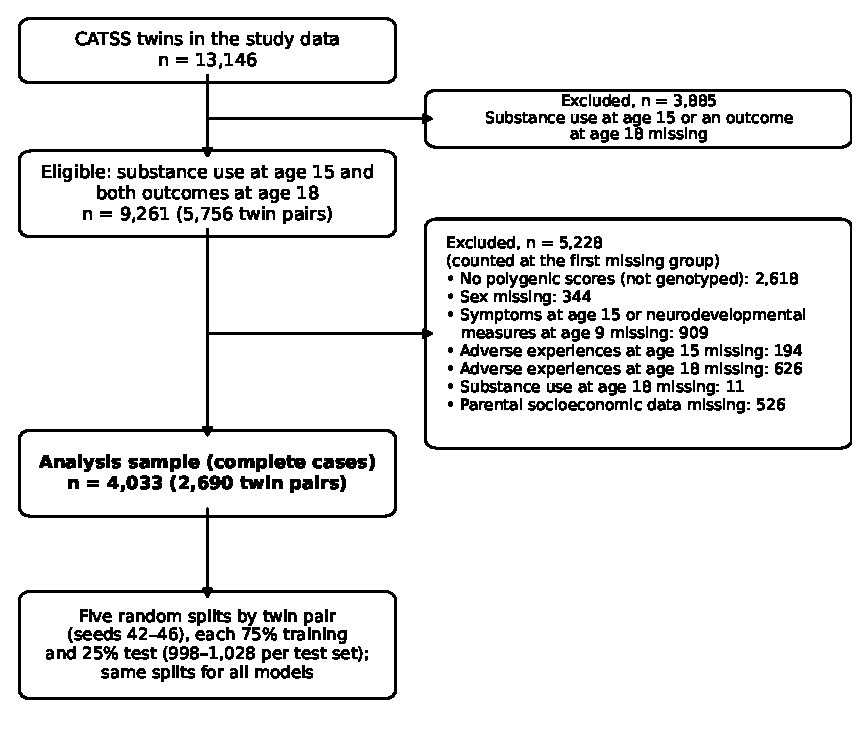
\includegraphics[width=\textwidth,height=0.85\textheight,keepaspectratio]{../figures/fig1_flow.pdf}
\clearpage
\noindent\textbf{Fig. 2}\par\medskip
\noindent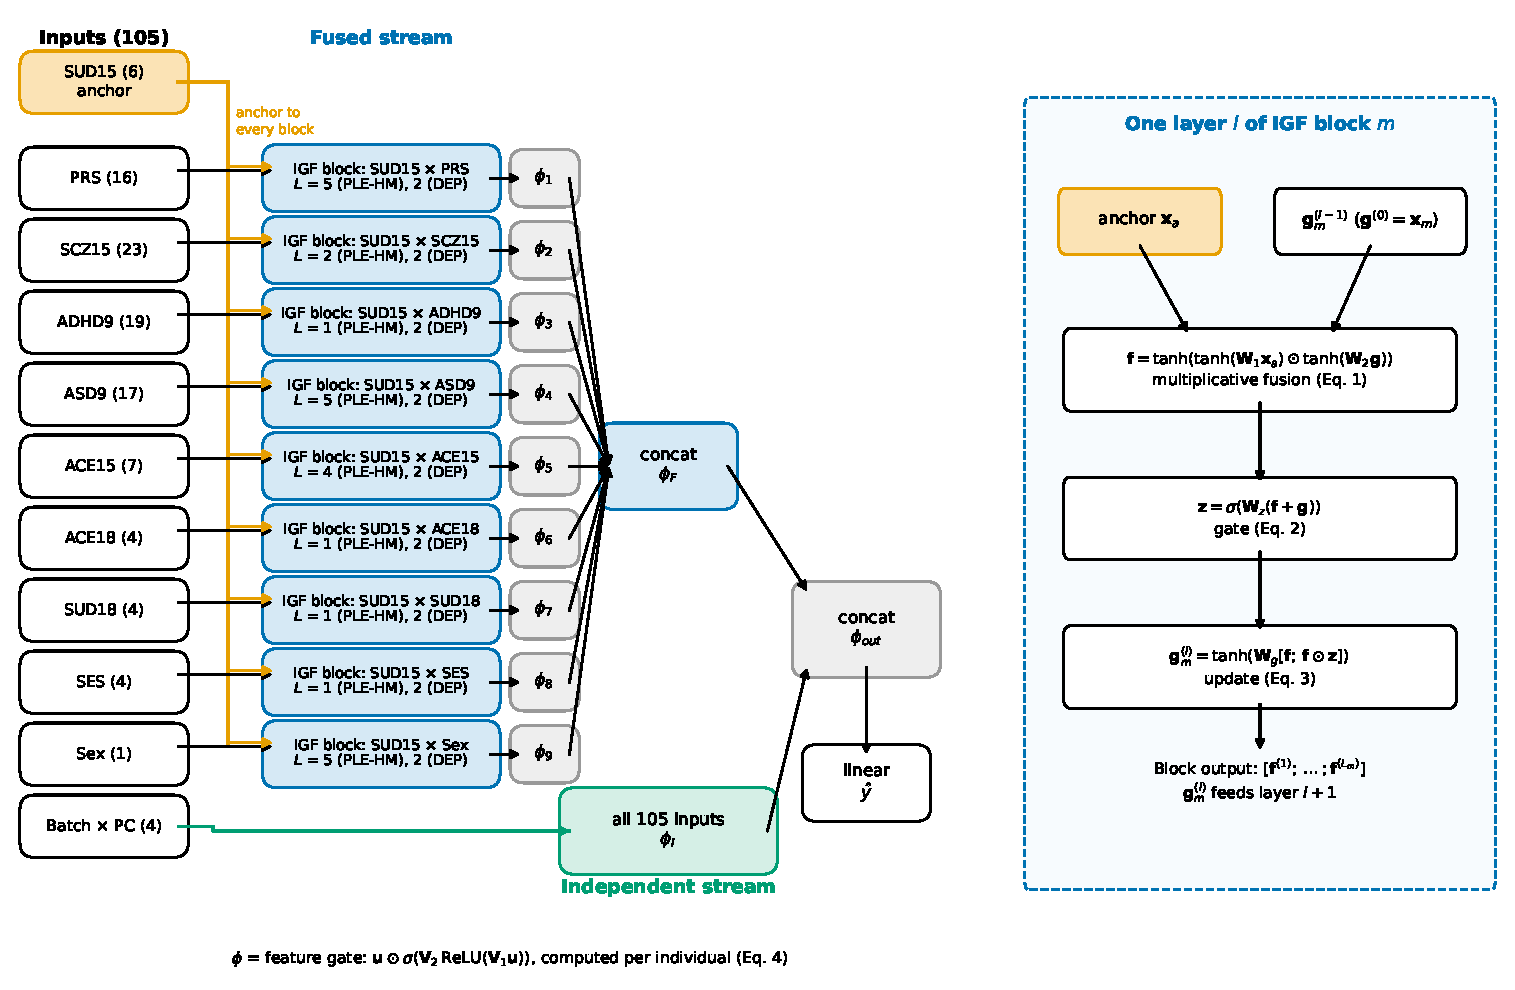
\includegraphics[width=\textwidth,height=0.85\textheight,keepaspectratio]{../figures/fig2_architecture.pdf}
\clearpage
\noindent\textbf{Fig. 3}\par\medskip
\noindent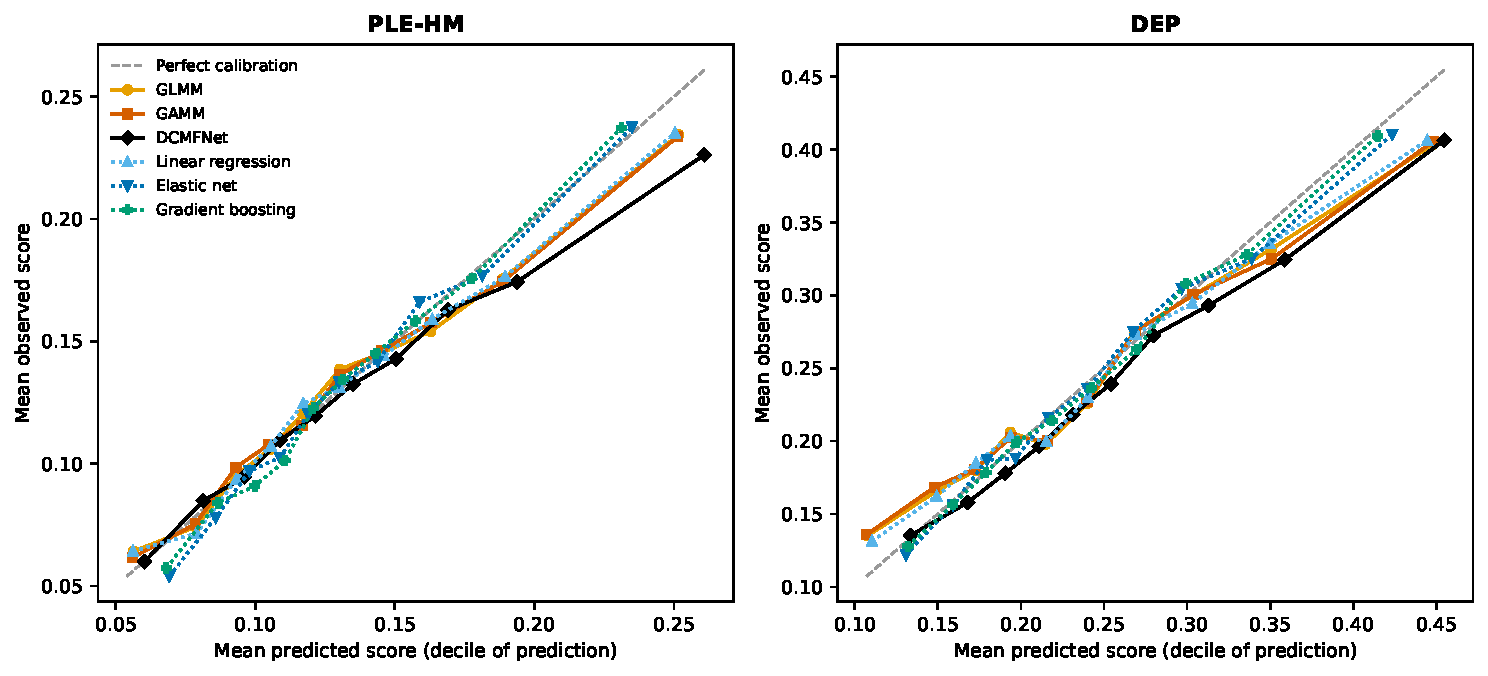
\includegraphics[width=\textwidth,height=0.85\textheight,keepaspectratio]{../figures/fig3_calibration.pdf}
\clearpage
\noindent\textbf{Fig. 4}\par\medskip
\noindent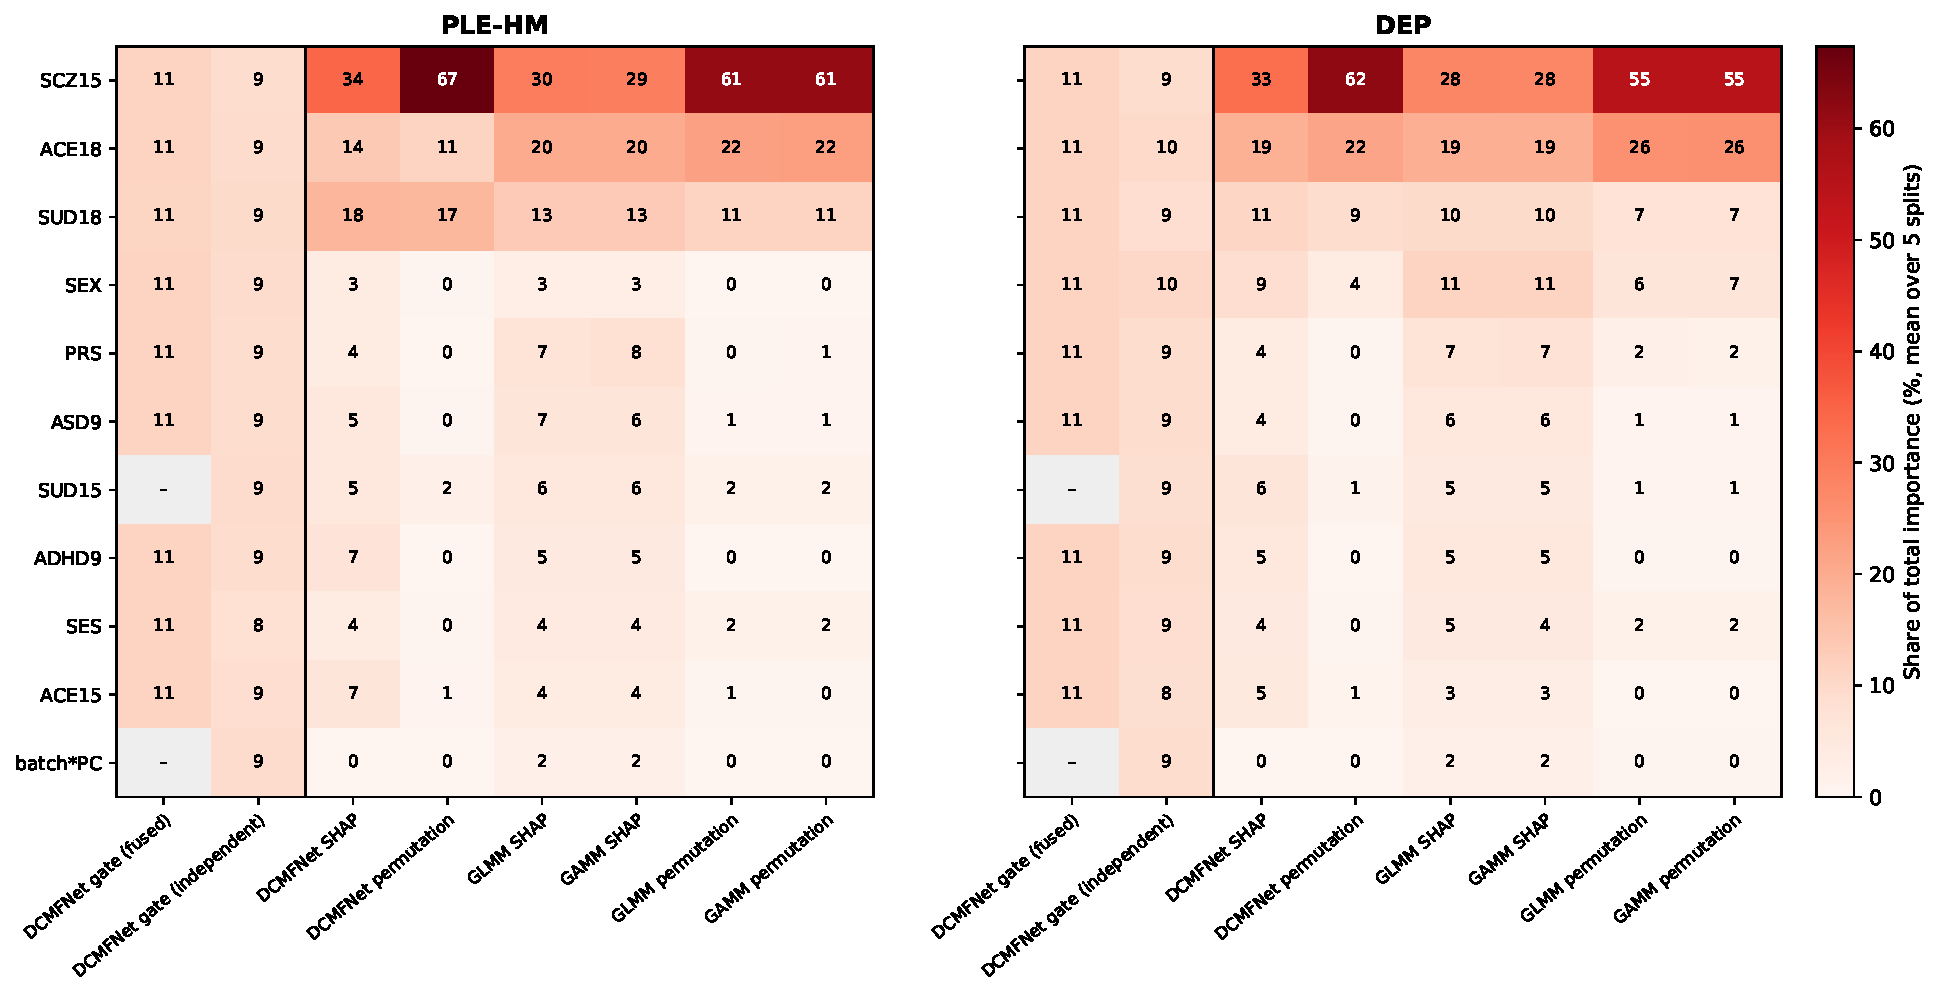
\includegraphics[width=\textwidth,height=0.85\textheight,keepaspectratio]{../figures/fig4_attribution.pdf}

\end{document}
